%-------------------------------------------------------------------------------
%                            BAB IV
%               		HASIL DAN PEMBAHASAN
%-------------------------------------------------------------------------------

\chapter{HASIL DAN PEMBAHASAN}
	\section{Analisis Kebutuhan}
	
	Hasil dari analisis kebutuhan yang telah dilakukan adalah mendapatkan persona, storyboard dan use case diagram untuk masing-masing pengguna.
	
	\subsection{Kelompok Pengguna}
	Kelompok pengguna dari aplikasi ini telah dapat diidentifikasikan pada tahap analisis kebutuhan pada sistem. terdapat 2 kelompok pengguna yang menggunakan aplikasi ini:
		 \begin{enumerate}[1.]
		 	\item Agen
		 		\newline Pengguna yang menggunakan aplikasi berbasis web untuk mengelola rencana penerimaan pasokan tabung ke pangkalan, melakukan rekapitulasi data penyaluran tabung pada pangkalan.
		 	\item Pangkalan
		 		\newline Pengguna yang menggunakan aplikasi berbasis android untuk melakukan pencatatan penjualan tabung per hari, mendaftarkan pelanggan baru, melakukan verifikasi pada penerimaan pasokan tabung.
		 \end{enumerate}
	 
	 Persona untuk masing-masing kelompok pengguna dapat dilihat pada lampiran 1
	
	\subsection{Storyboard}
	Dengan menggunakan \textit{Storyboard} kita dapat memetakan secara visual kegiatan pengguna sebelum dan sesudah menggunakan aplikasi. Berdasarkan hasil pengamatan dan analisis kebutuhan dapat digambarkan \textit{Storyboard} seperti berikut:
	
	\vspace{-0.4cm}
	\begin{figure}[H]
		\center
		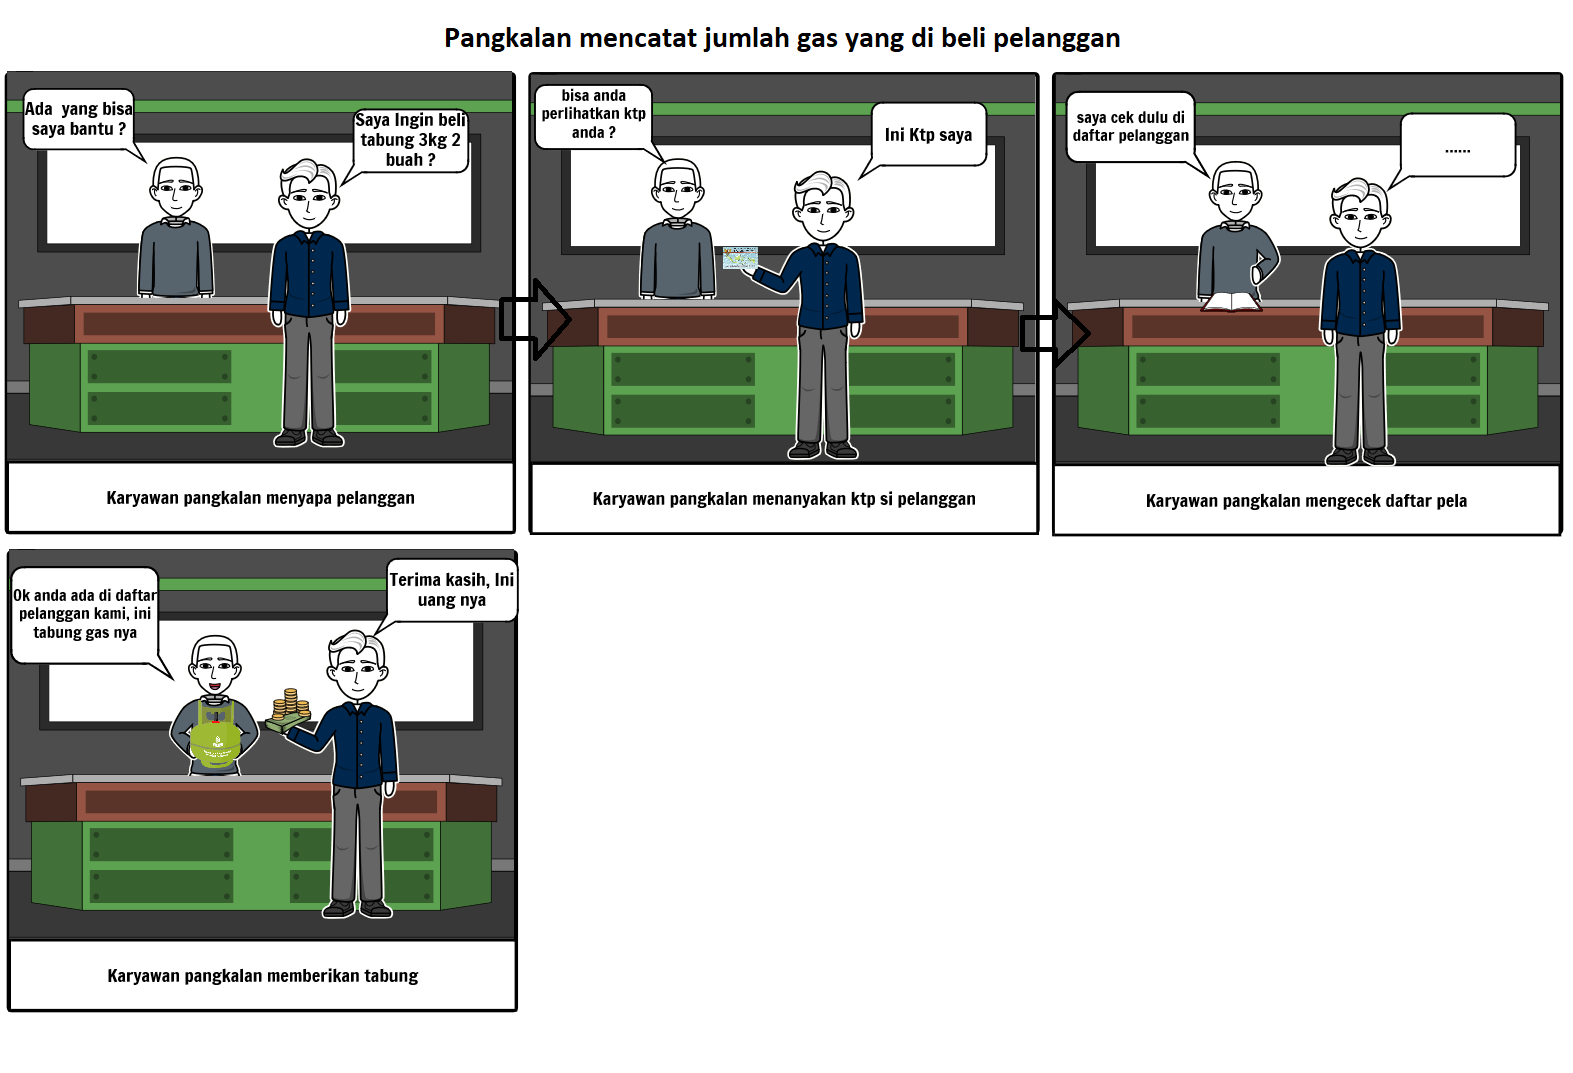
\includegraphics [width = 14cm]{gambar/storyboard/storyboard-1-(old)}
		\caption{Kegiatan Sebelum Menggunakan Aplikasi}
		\label{storyboardOld1}
	\end{figure}
	
	\begin{figure}[H]
		\center
		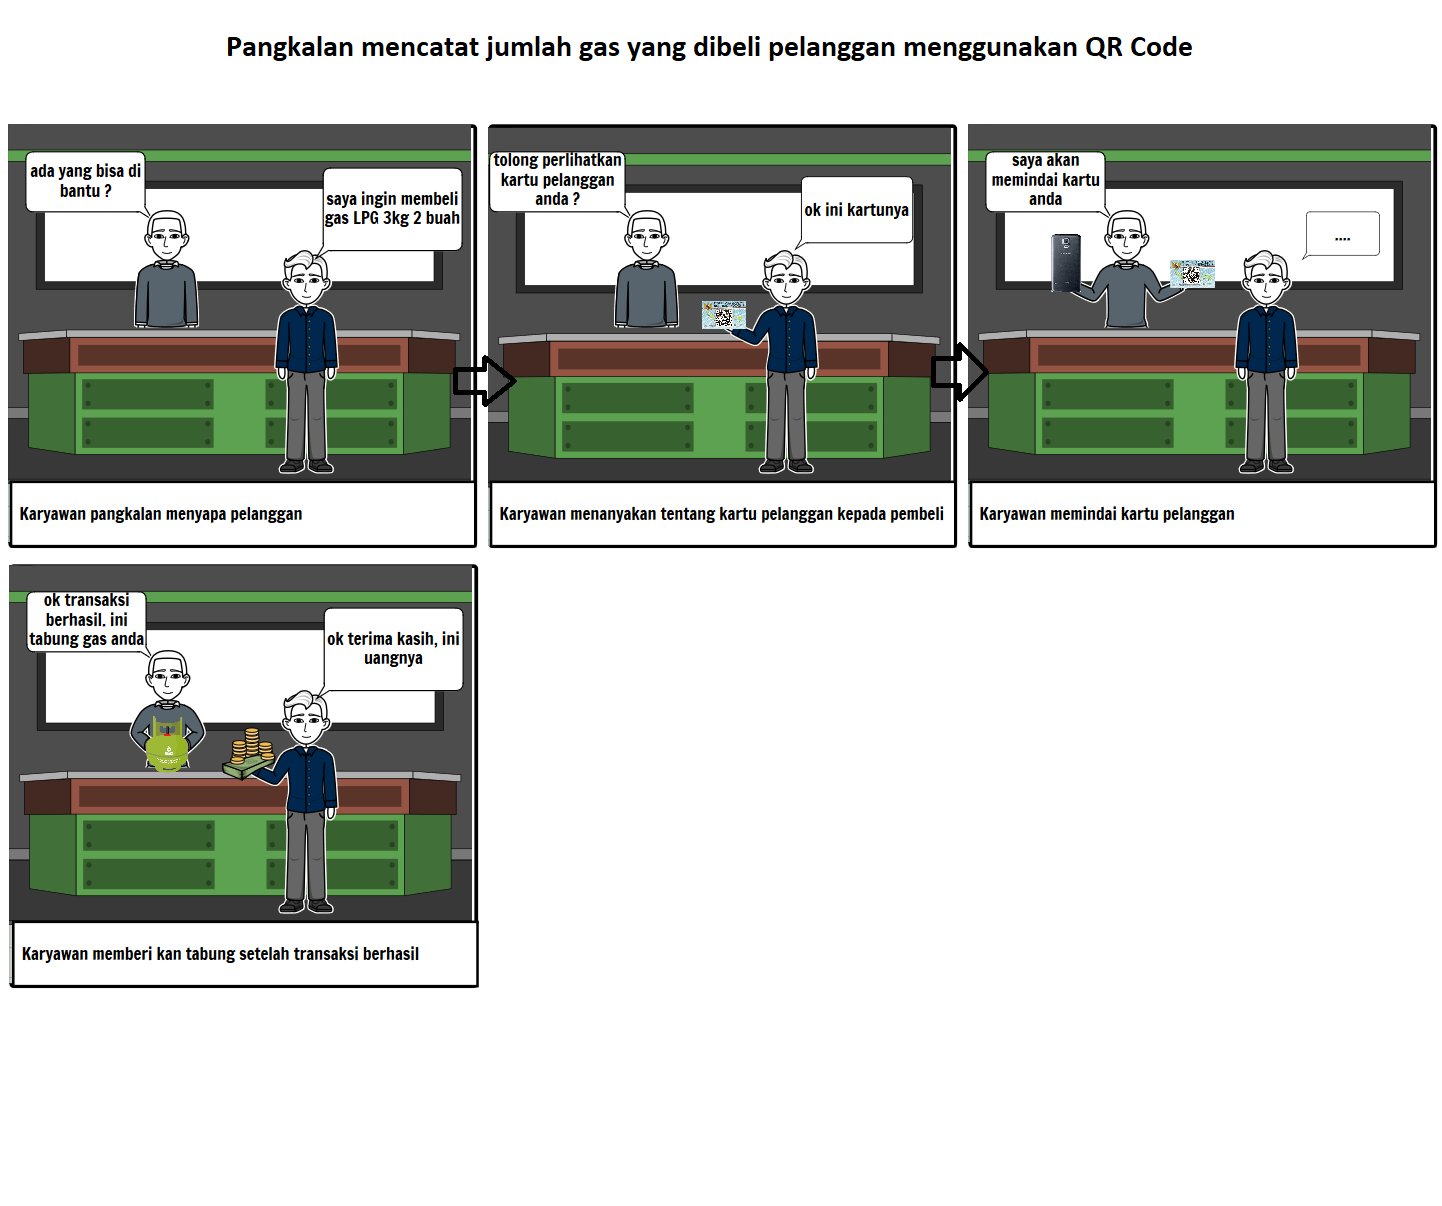
\includegraphics [width = 14cm]{gambar/storyboard/storyboard-1-(new)}
		\caption{Kegiatan Sesudah Menggunakan Aplikasi}
		\label{storyboardNew1}
	\end{figure}
	
	
	
	\subsection{\textit{Value Proposition Canvas }(VPC)}
	Dengan Menggunakan \textit{Value Proposition Canvas} (VPC) ini, kita dapat menguji apakah desain aplikasi dan fitur-fiturnya telah memenuhi kebutuhan dari pengguna aplikasi. Dari hasil pengamatan yang telah dilakukan maka dapat digambarkan VPC sebagai berikut:
	
		\vspace{-0.4cm}
	\begin{figure}[H]
		\center
		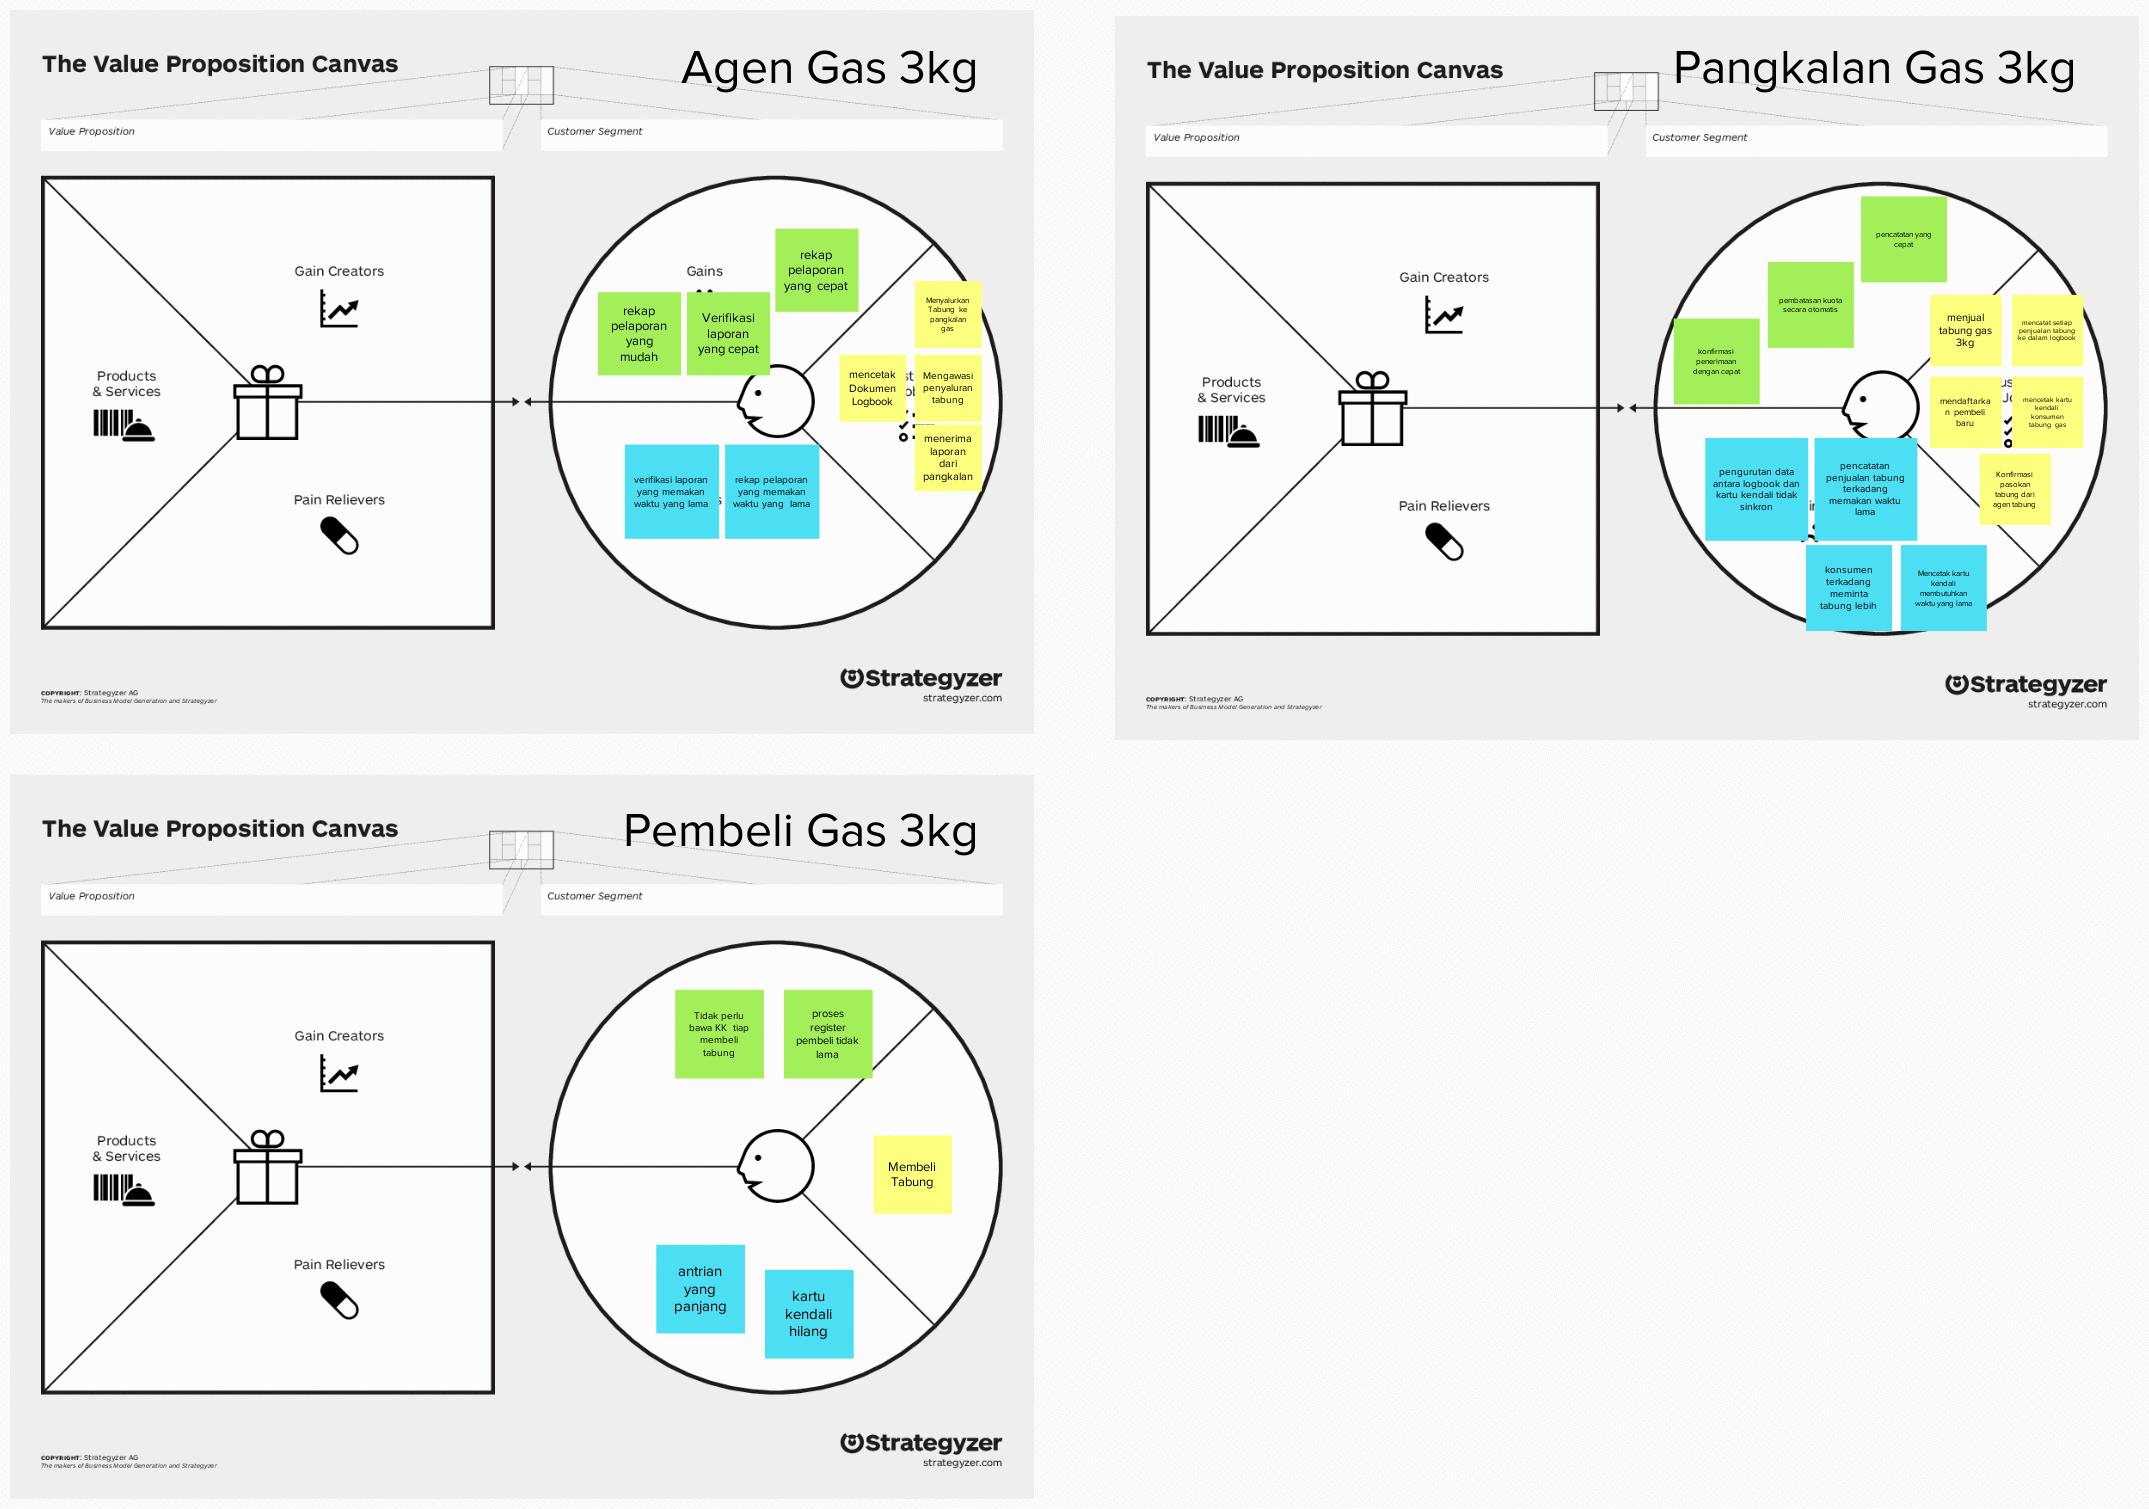
\includegraphics [width = 14cm]{gambar/model/VPC-Gas}
		\caption{Kegiatan Sebelum Menggunakan Aplikasi}
		\label{vpc}
	\end{figure}

	
	\subsection{\textit{Use Case}}
	\textit{Use-Case Diagram} digunakan untuk memetakan fungsionalitas aplikasi pada masing-masing pengguna. Dari hasil pengamatan dapat digambarkan \textit{Use-Case Diagram} sebagai berikut:
	
	\vspace{-0.4cm}
	\begin{figure}[H]
		\center
		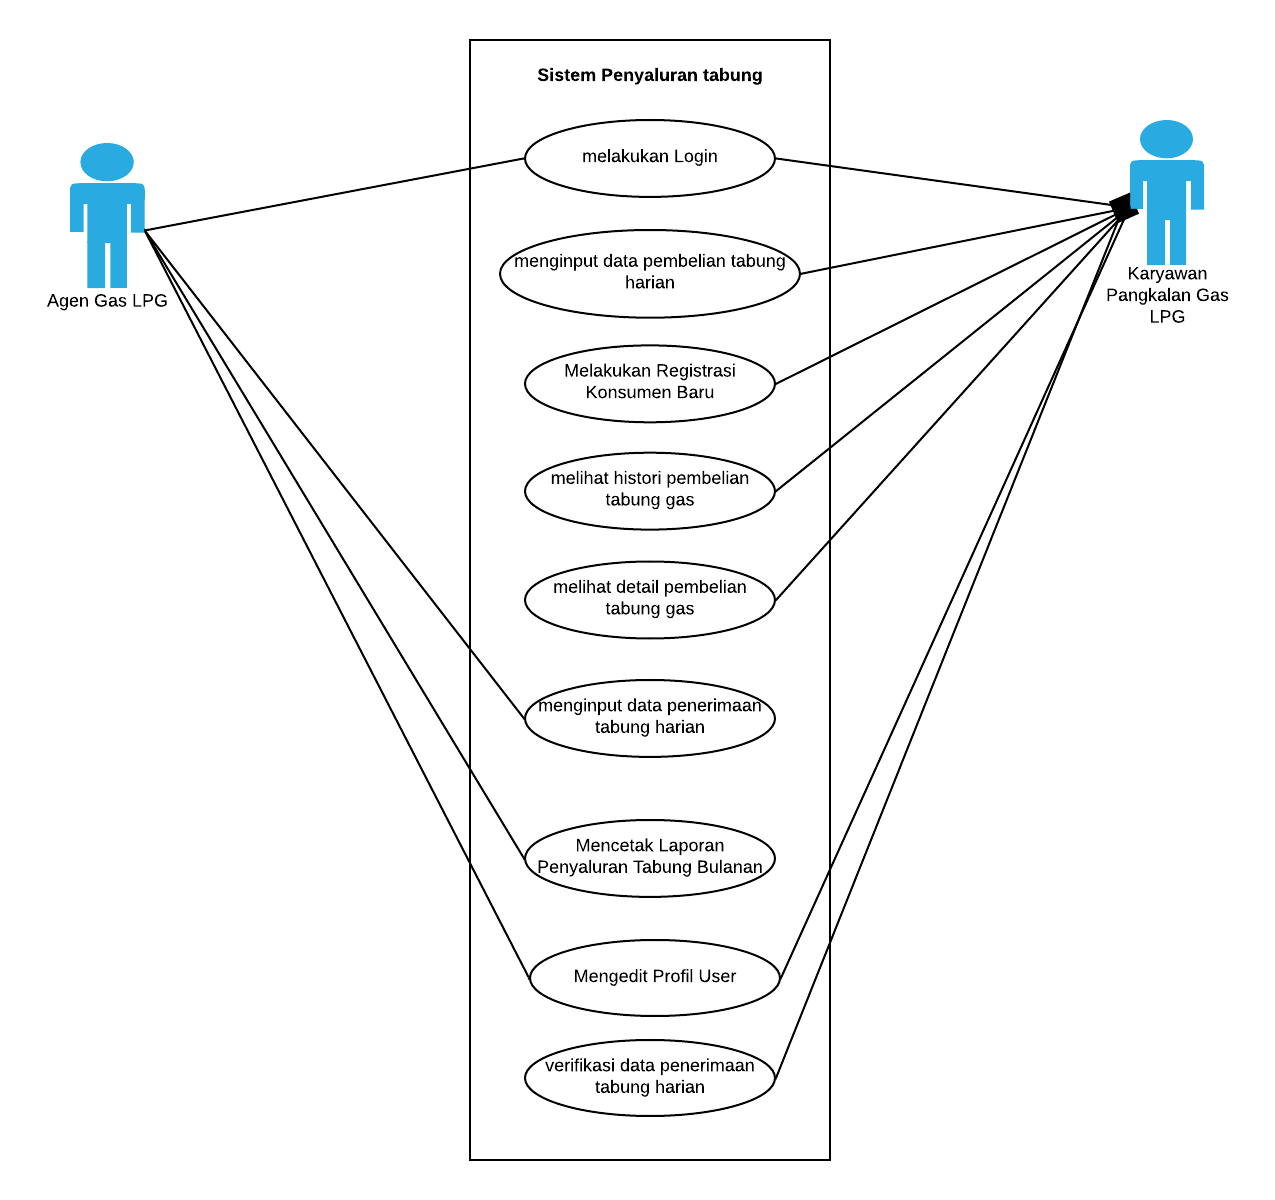
\includegraphics [width = 14cm]{gambar/model/use-case-diagram}
		\caption{Use-Case Diagram}
		\label{usecase}
	\end{figure}
	
	\section{Desain dan Pembuatan Sistem}
	
	\subsection{Desain Sistem}
	\par Desain Sistem adalah proses desain pada aplikasi yang akan dibangun. proses dilakukan berdasarkan proses analisis kebutuhan aplikasi yang telah dilakukan pada proses sebelumnya. proses ini terdiri dari beberapa tahap yaitu seperti perancangan \textit{deployment diagram},
	perancangan arsitektur aplikasi dalam bentuk \textit{component diagram}, perancangan struktur basis data dalam bentuk \textit{class diagram}, dan juga perancangan tampilan antar muka dari aplikasi yang akan dibangun.
	
	\par tahap pertama adalah merancang \textit{deployment diagram}, dimana \textit{deployment diagram} adalah diagram yang menjelaskan bagaimana sistem aplikasi akan bekerja dan digunakan oleh pengguna. aplikasi yang dibangun terdiri dari 2 platform yang berbeda dimana pengguna pangkalan akan menggunakan platform android untuk melakukan pencatatan penjualan tabung, dan lain-lain, sedangkan pengguna agen akan menggunakan platform \textit{web-based} untuk rekapitulasi laporan penyaluran. Berikut rancangan \textit{deployment diagram} yang telah dibuat:
	
		\vspace{-0.4cm}
	\begin{figure}[H]
		\center
		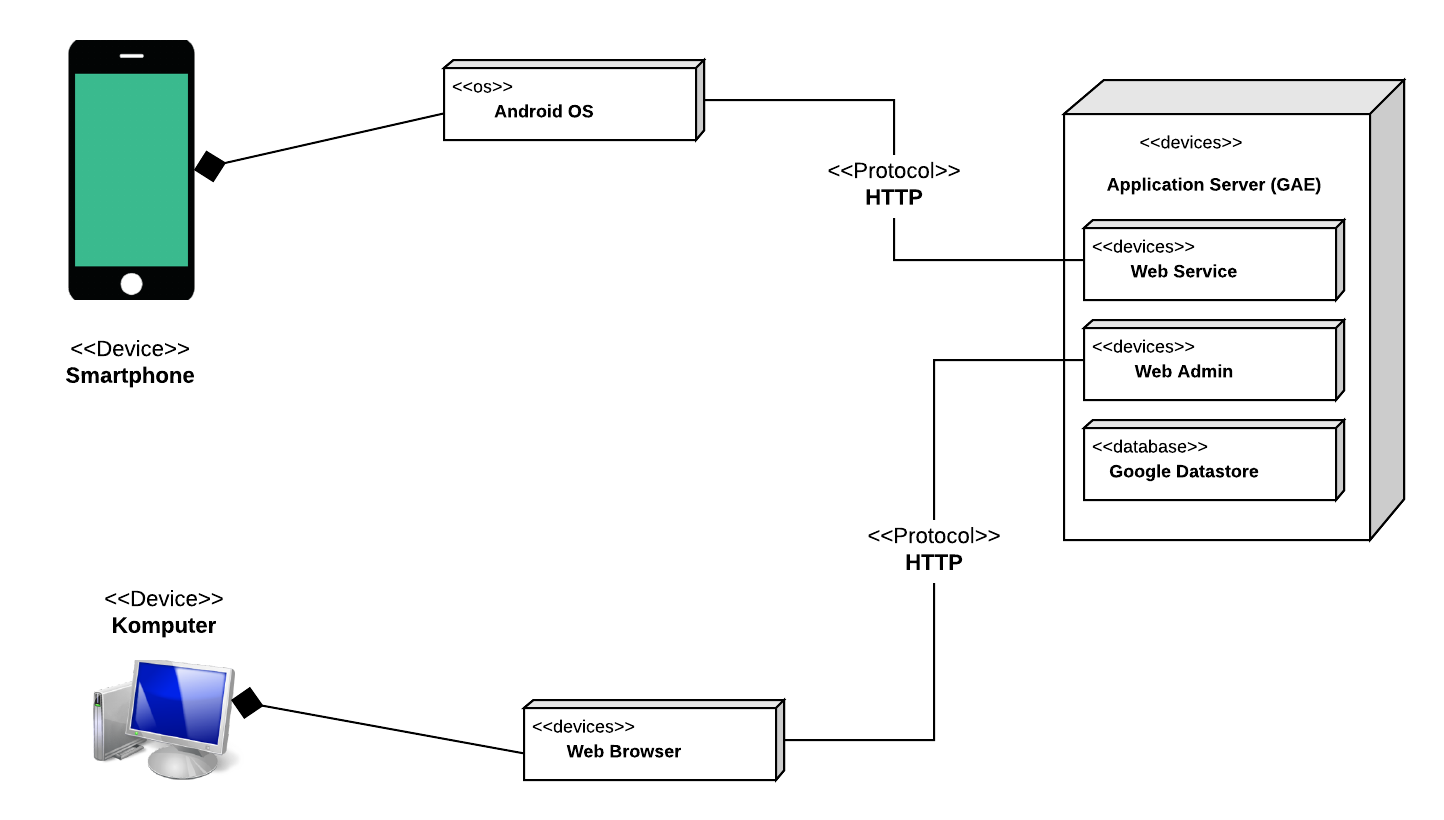
\includegraphics [width = 14cm]{gambar/model/deployment}
		\caption{Diagram Deployment}
		\label{deployment}
	\end{figure}

	\par tahap selanjutnya adalah merancang \textit{component diagram}, dimana \textit{component diagram} adalah diagram yang menjelaskan arsitektur sistem aplikasi yang akan dibangun secara keseluruhan. Berikut rancangan \textit{component diagram} yang telah dibuat:
	
	\vspace{-0.4cm}
	\begin{figure}[H]
		\center
		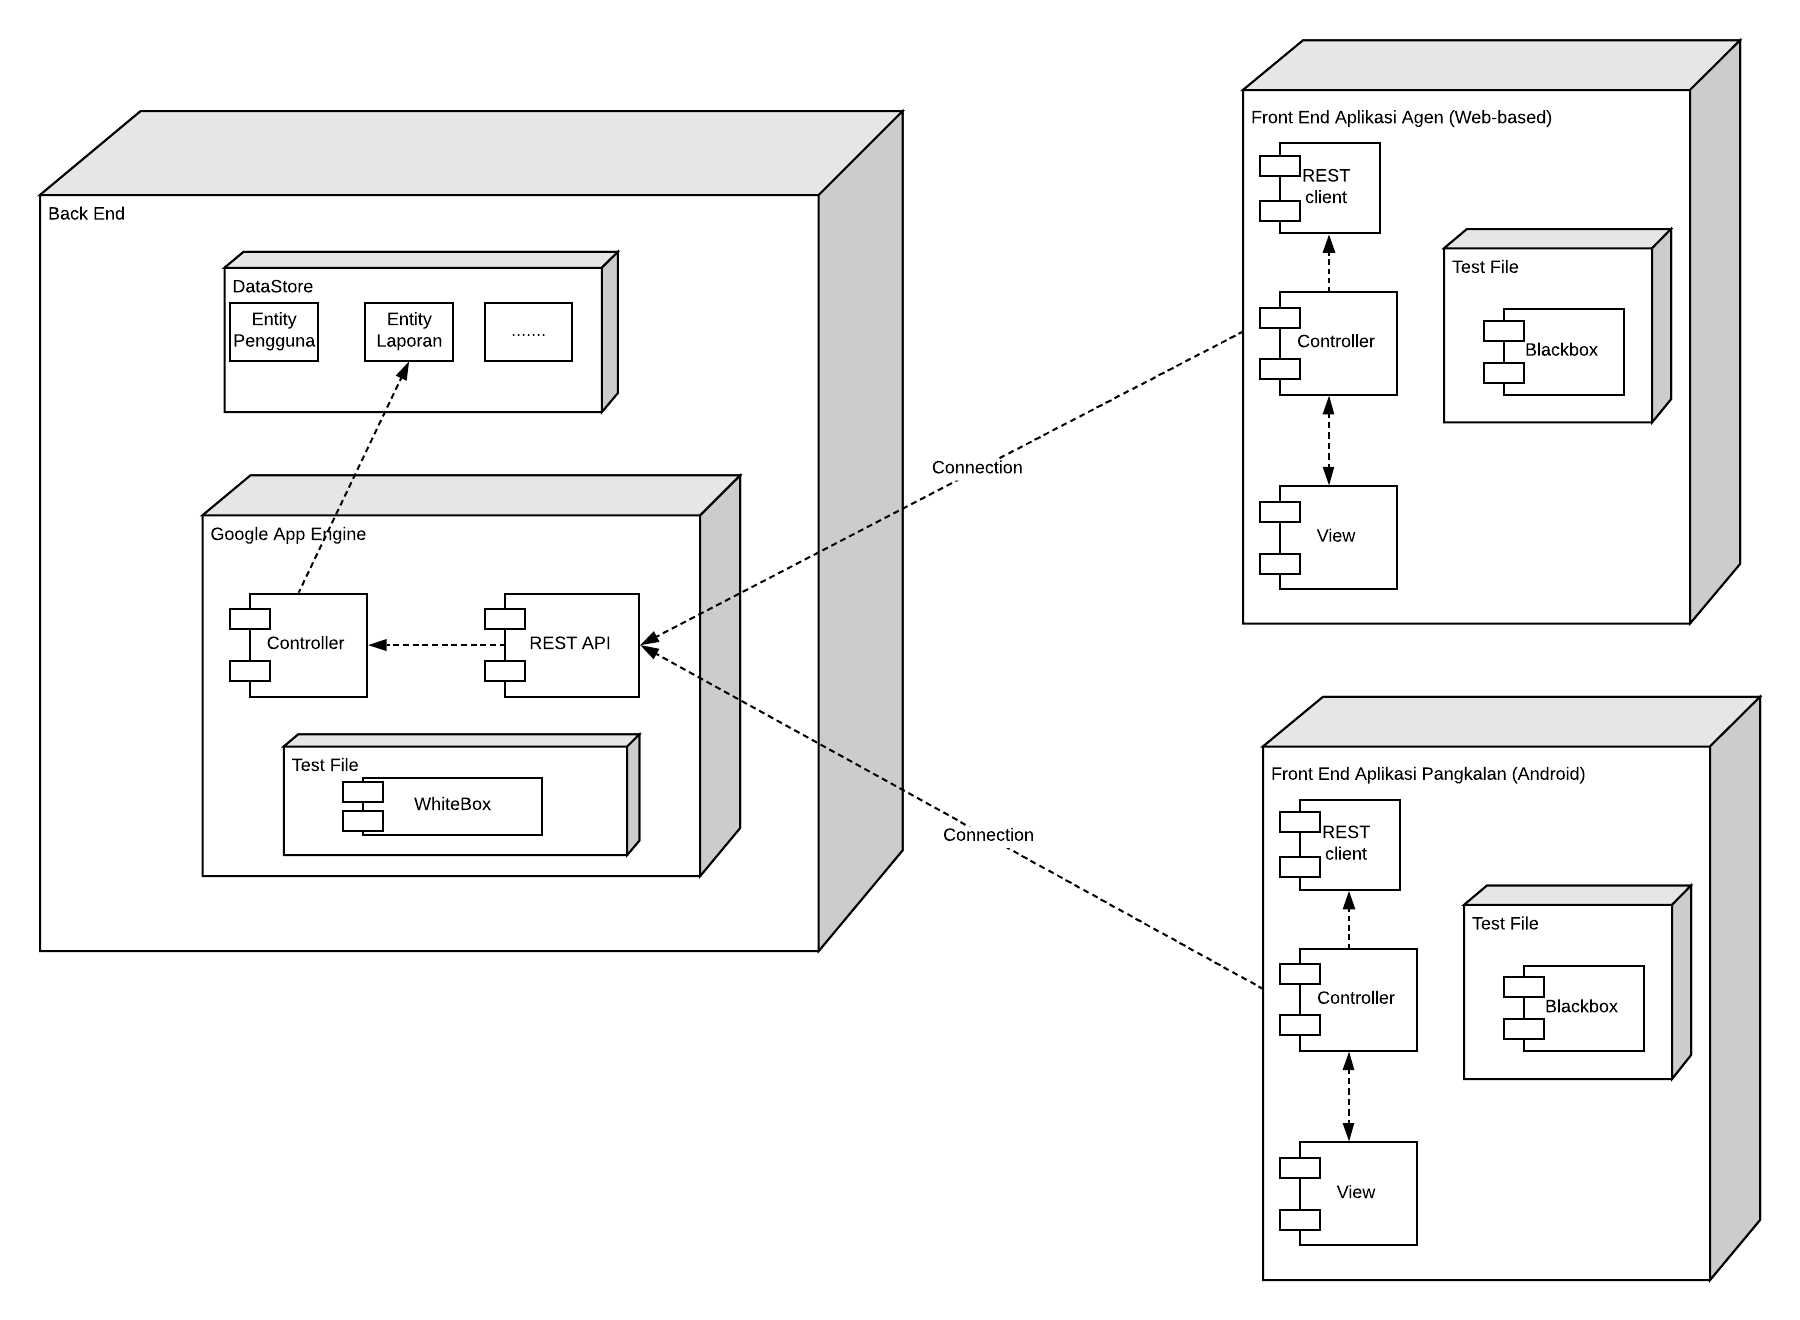
\includegraphics [width = 14cm]{gambar/model/component}
		\caption{Diagram Component}
		\label{component}
	\end{figure}

	\pagebreak
	\par Dilanjutkan dengan tahap perancangan model basis data menggunakan \textit{class diagram}. diagram ini dibuat berdasarkan fungsionalitas dari sistem yang akan dibangun. Berikut rancangan \textit{class diagram} yang telah dibuat:
	
		\vspace{-0.4cm}
	\begin{figure}[H]
		\center
		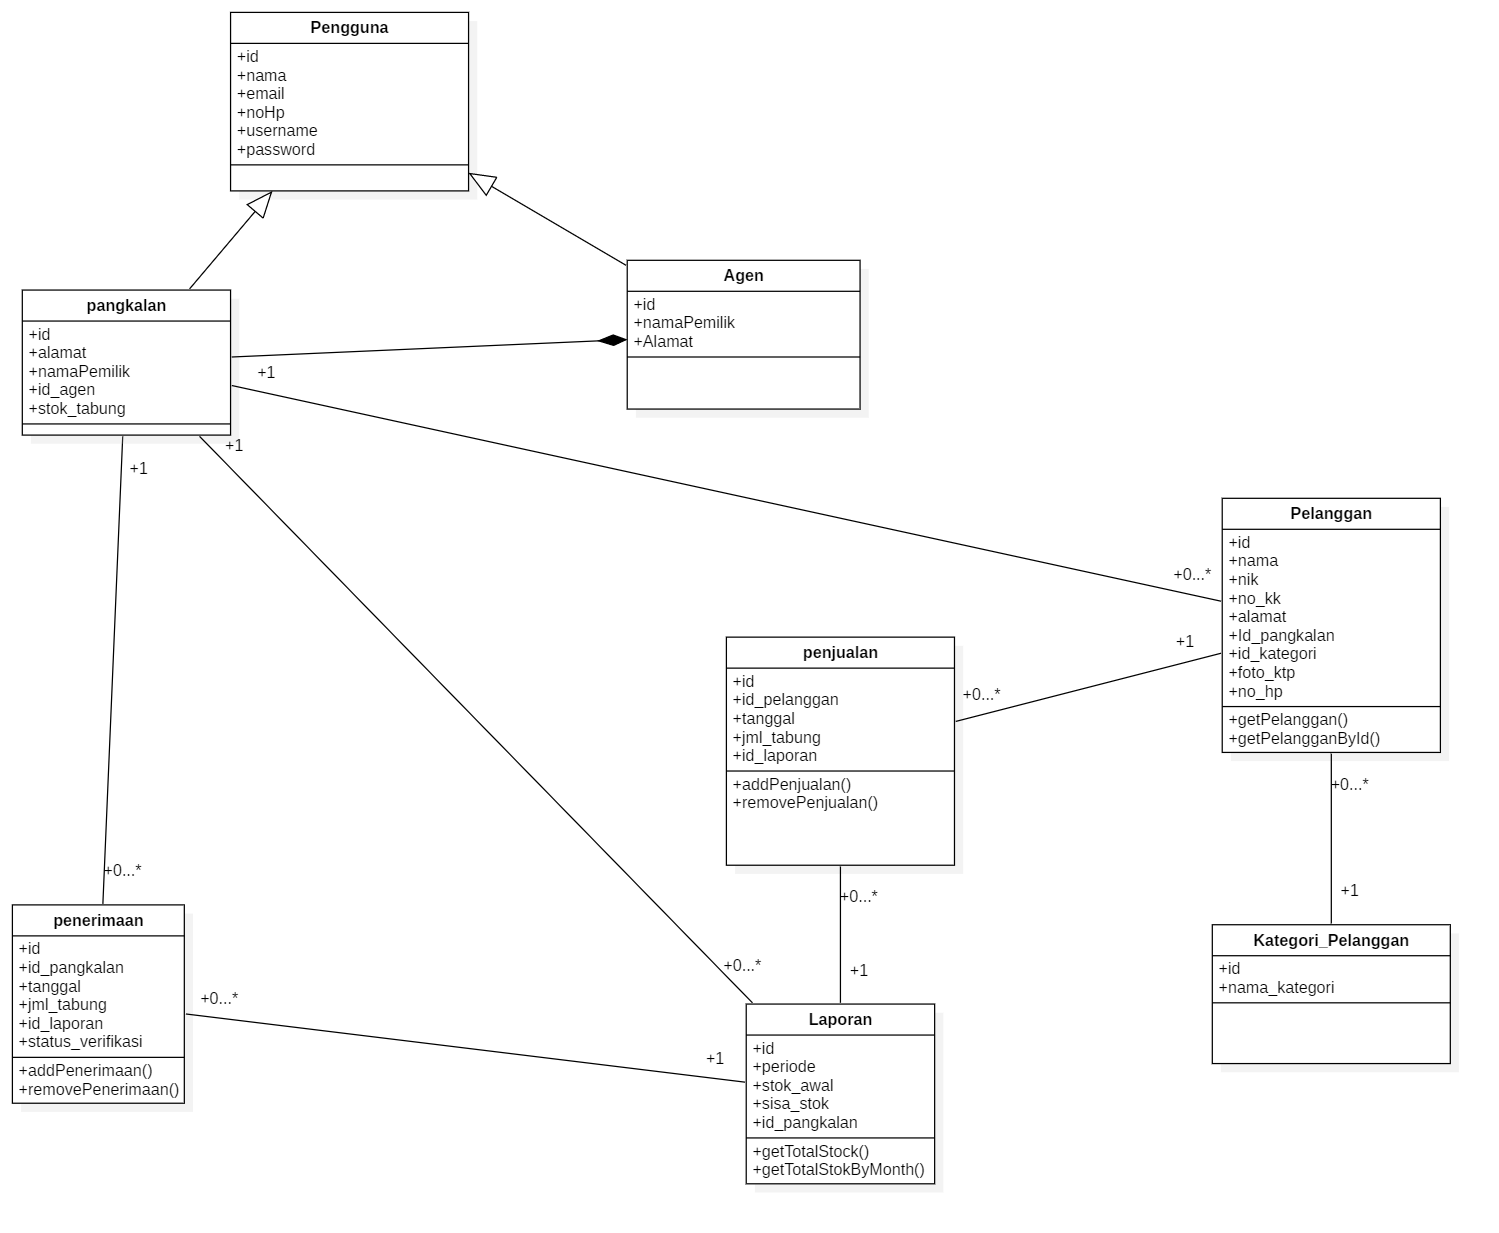
\includegraphics [width = 14cm]{gambar/model/class-diagram}
		\caption{Diagram Kelas Model Basis Data }
		\label{class}
	\end{figure}

	\par Selanjutnya adalah perancangan layanan web, perancangan layanan web disini memiliki peran yang sangat penting dan vital, dimana layanan web harus dapat menangani setiap proses transaksi data yang dilakukan oleh sistem. layanan web ini menggunakan RESTful API untuk dapat berinteraksi dengan \textit{platform} android dan aplikasi lain melalui HTTP URL.
	
	\par Untuk perancangan antar muka dari aplikasi ini menggunakan ionic framework karena menyediakan komponen-komponen antar muka pengguna seperti \textit{tabs, card, dan button} yang cocok untuk digunakan pada platform \textit{mobile}.
	
	\par Tampilan Aplikasi berbasis android untuk pangkalan gas LPG 3Kg ini terdiri 3 halaman utama yaitu halaman register pelanggan baru, halaman pembelian tabung, dan halaman penerimaan tabung. Pertama-tama untuk masuk ke dalam aplikasi, pangkalan harus melakukan \textit{login} menggunakan no HP yang telah terdaftar seperti pada gambar \ref{tampilanLoginPangkalan}. setelah itu akan muncul sms no HP tersebut berisi sebuah kode OTP(\textit{One Time Password}) yang digunakan untuk verifikasi no HP valid atau tidak. setelah proses \textit{login} berhasil maka dilanjut ke halaman beranda yang berisi menu utama aplikasi seperti pada Gambar \ref{tampilanBerandaPangkalan}.
	\par Pada halaman registrasi pelanggan baru terdapat \textit{form} mengenai data pelanggan setelah itu dilanjutkan pengambilan foto ktp dan foto diri pelanggan seperti pada Gambar \ref{tampilanRegisterPangkalan}. Pada saat pembelian tabung, pangkalan harus mencari pelanggan terlebih dahulu menggunakan NIK (Nomor Induk Kependudukan) seperti pada Gambar \ref{tampilanPembelianPangkalan} setelah itu maka akan muncul halaman detail pelanggan berisi detail data pelanggan tersebut. pada halaman ini terdapat 2 tombol aksi yaitu riwayat pembelian dan beli tabung seperti pada Gambar \ref{tampilanPembelianPangkalan}. setelah pangkalan memilih beli tabung selanjutnya pangkalan harus memilih jumlah tabung yang dibeli dan dilanjutkan pengambilan foto pembeli sebagai bukti pembelian seperti pada Gambar \ref{tampilanPembelianPangkalan}. Pada saat penerimaan pasokan tabung, pangkalan harus melakukan verifikasi penerimaan tabung pada menu penerimaan tabung seperti pada Gambar \ref{tampilanPenerimaanPangkalan}.
	
	\vspace{-0.2cm}
	\begin{figure}[H]
		\center
		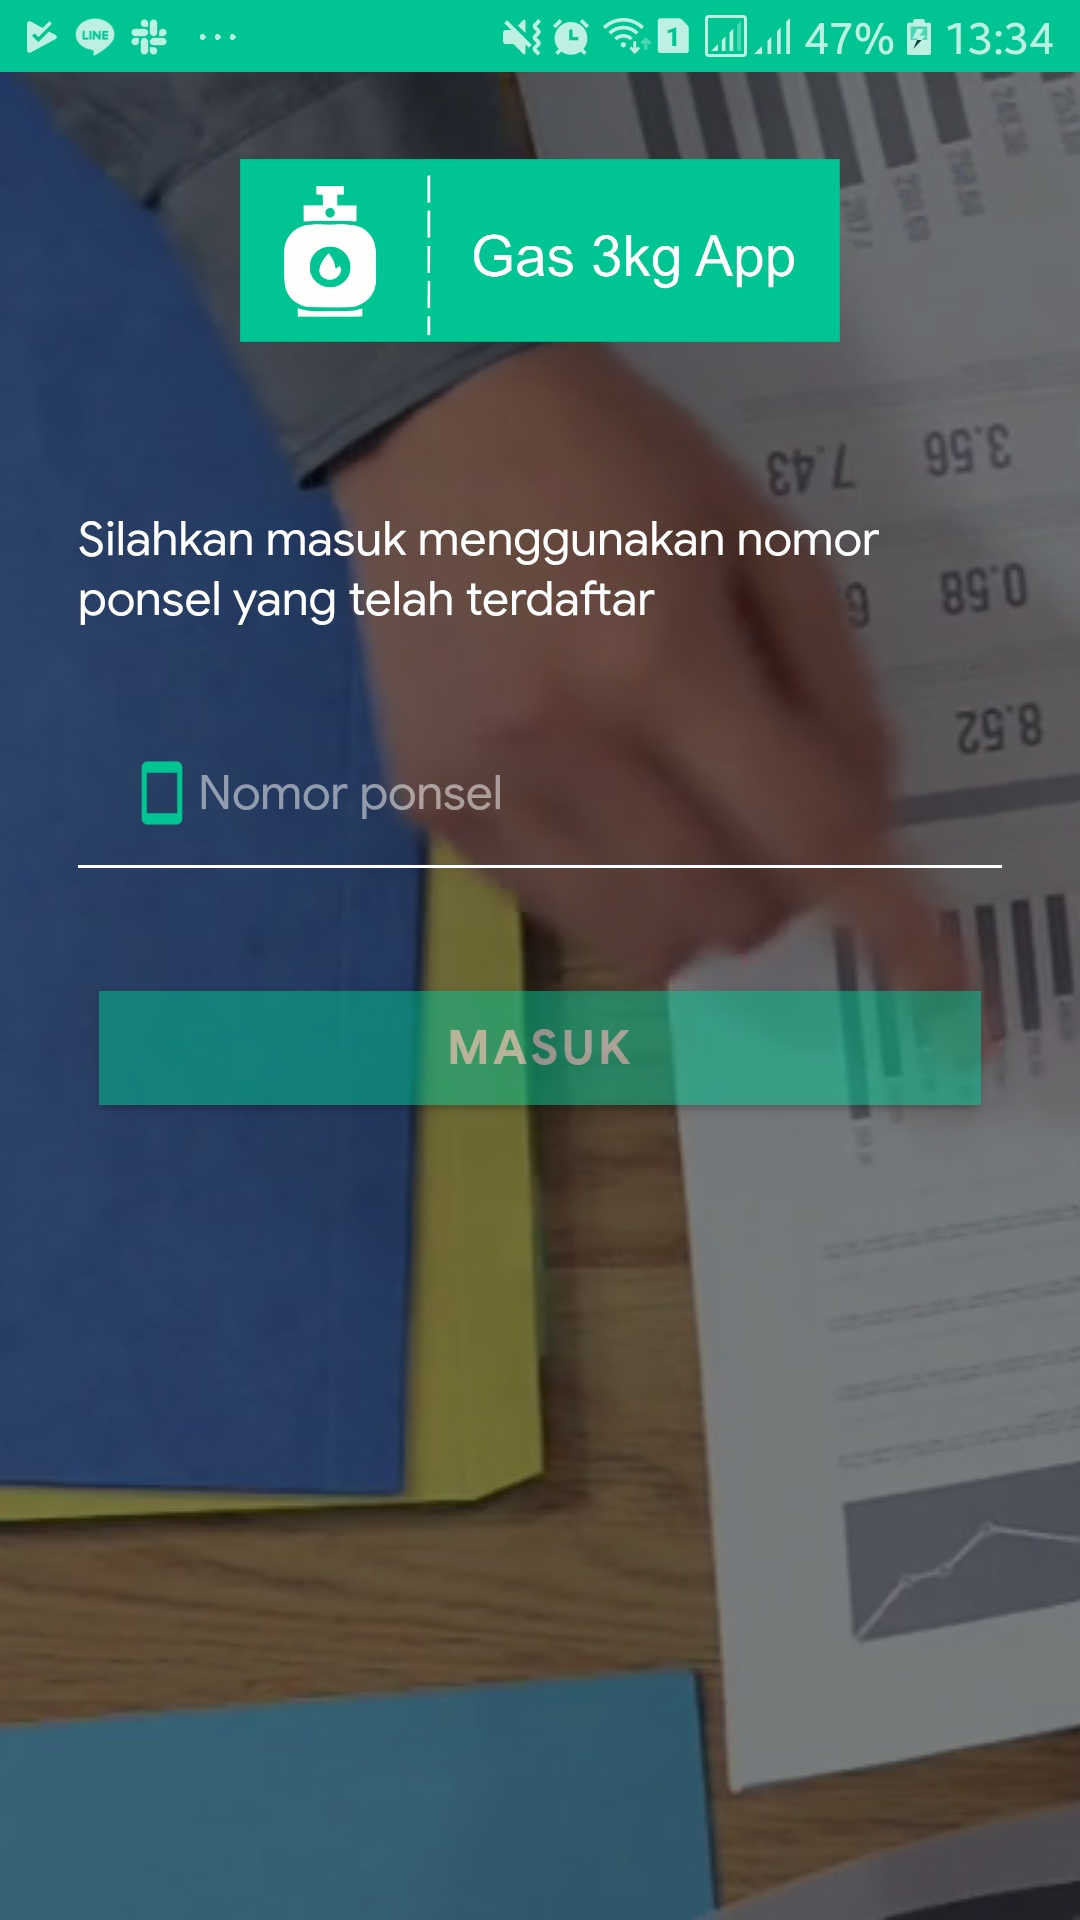
\includegraphics [width = 7cm]{gambar/android/login}
		\vspace{1cm}
		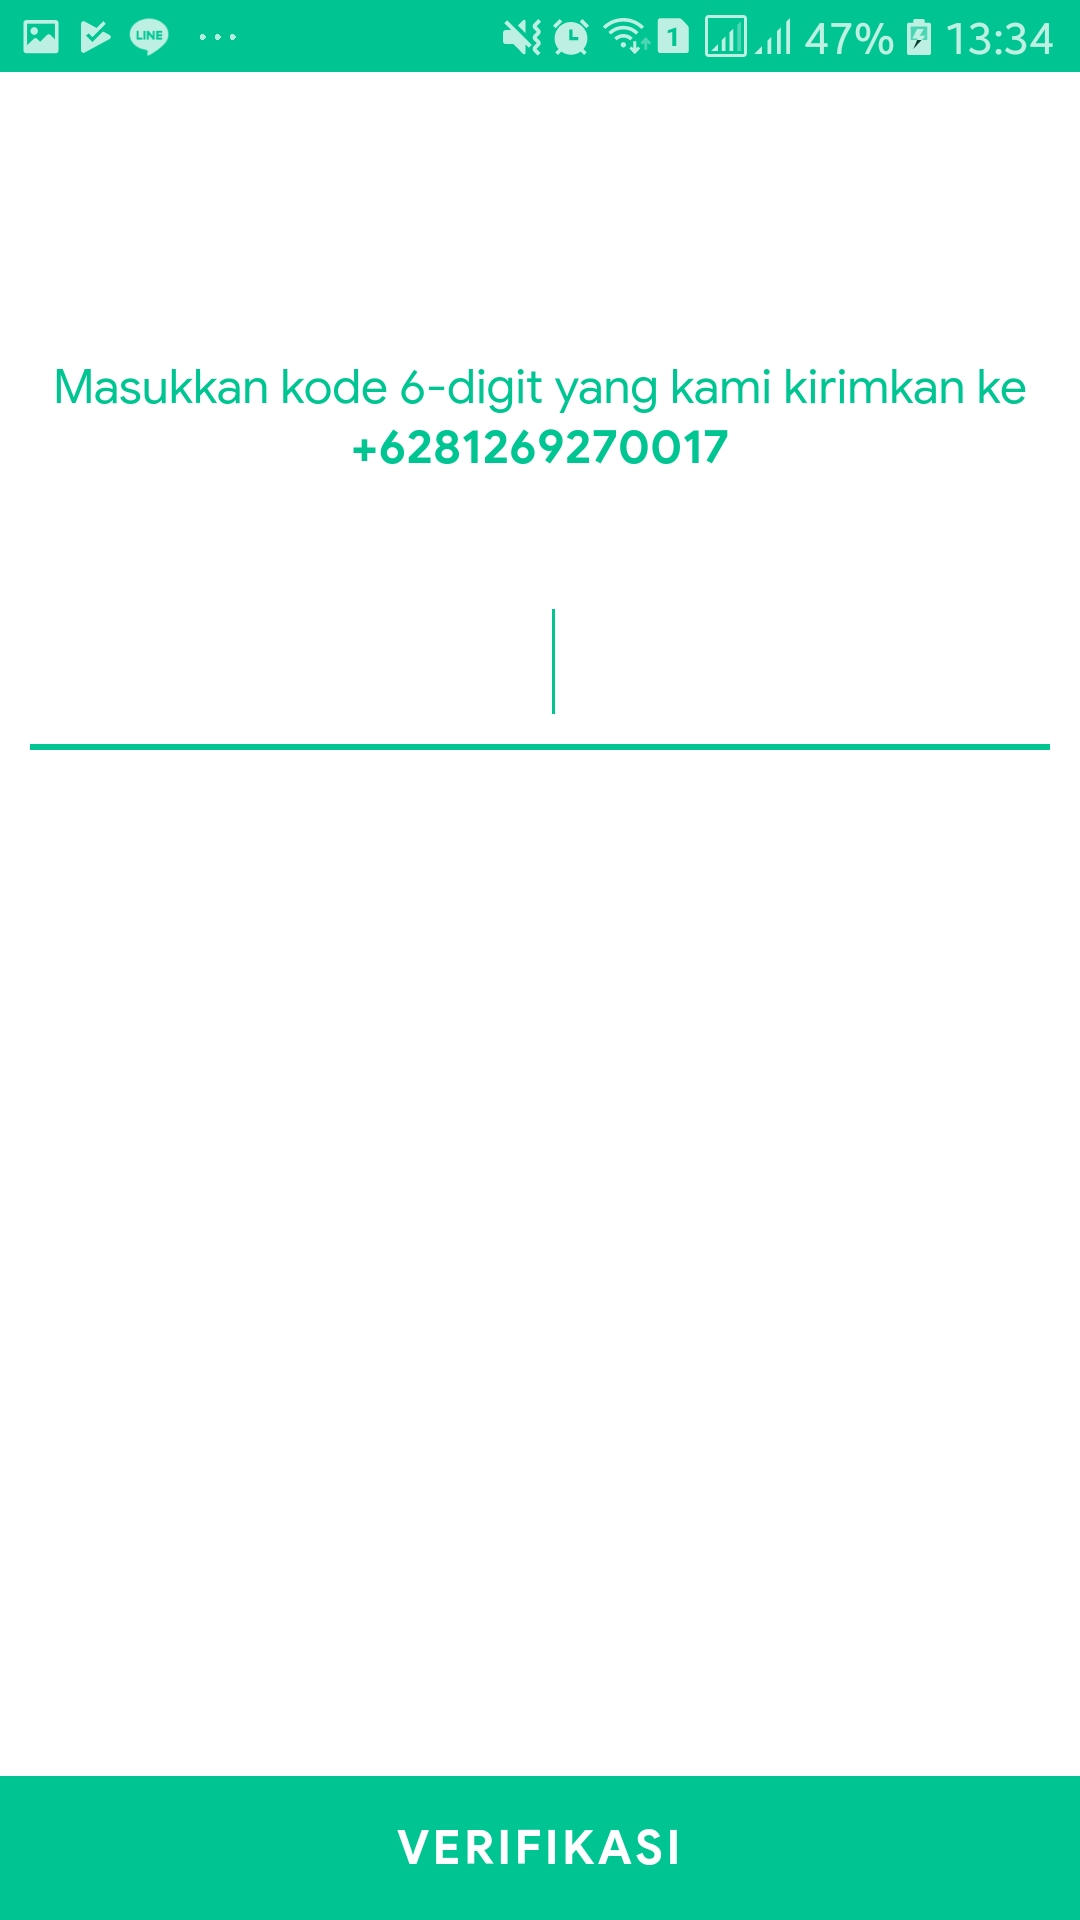
\includegraphics [width = 7cm]{gambar/android/verify}
		\caption{Tampilan Login aplikasi}
		\label{tampilanLoginPangkalan}
	\end{figure}
	
	\begin{figure}[H]
		\center
		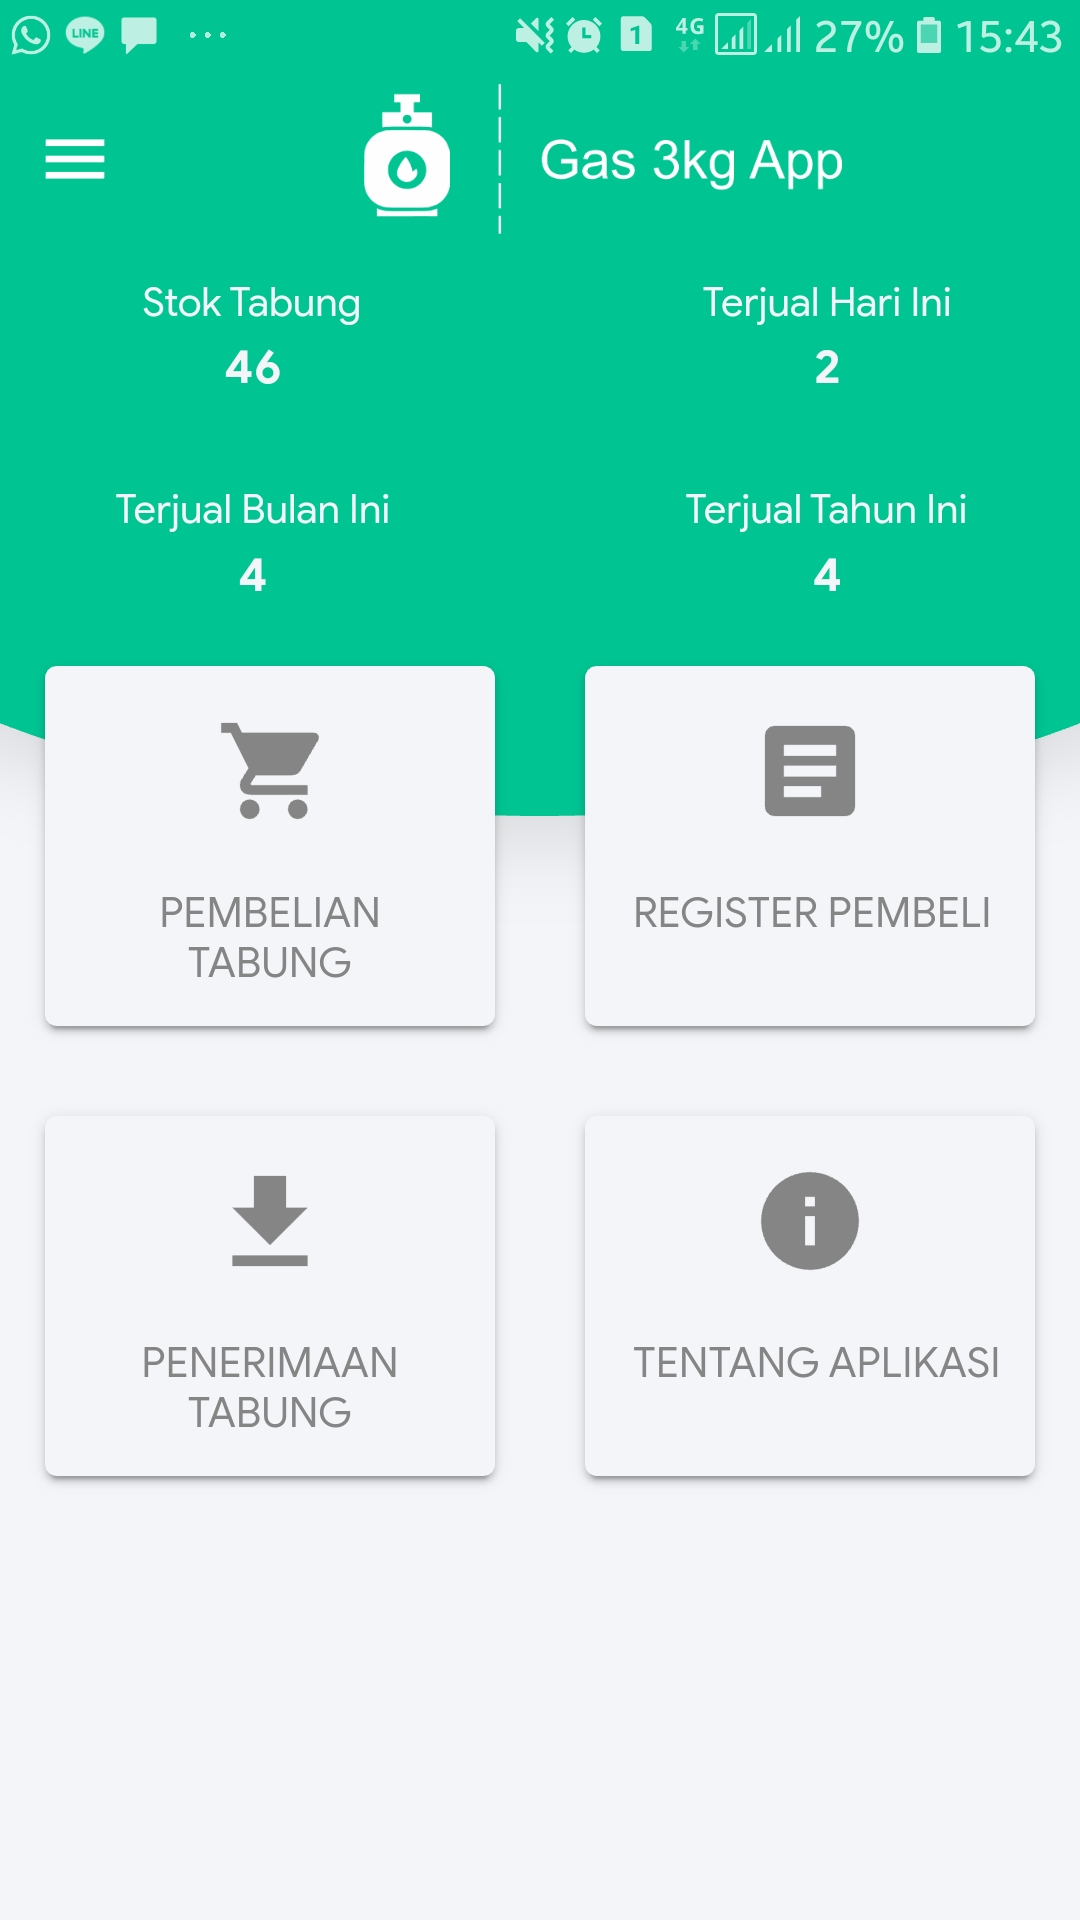
\includegraphics [width = 7cm]{gambar/android/beranda}
		\caption{Tampilan Halaman Beranda}
		\label{tampilanBerandaPangkalan}
	\end{figure}

	\begin{figure}[H]
		\center
		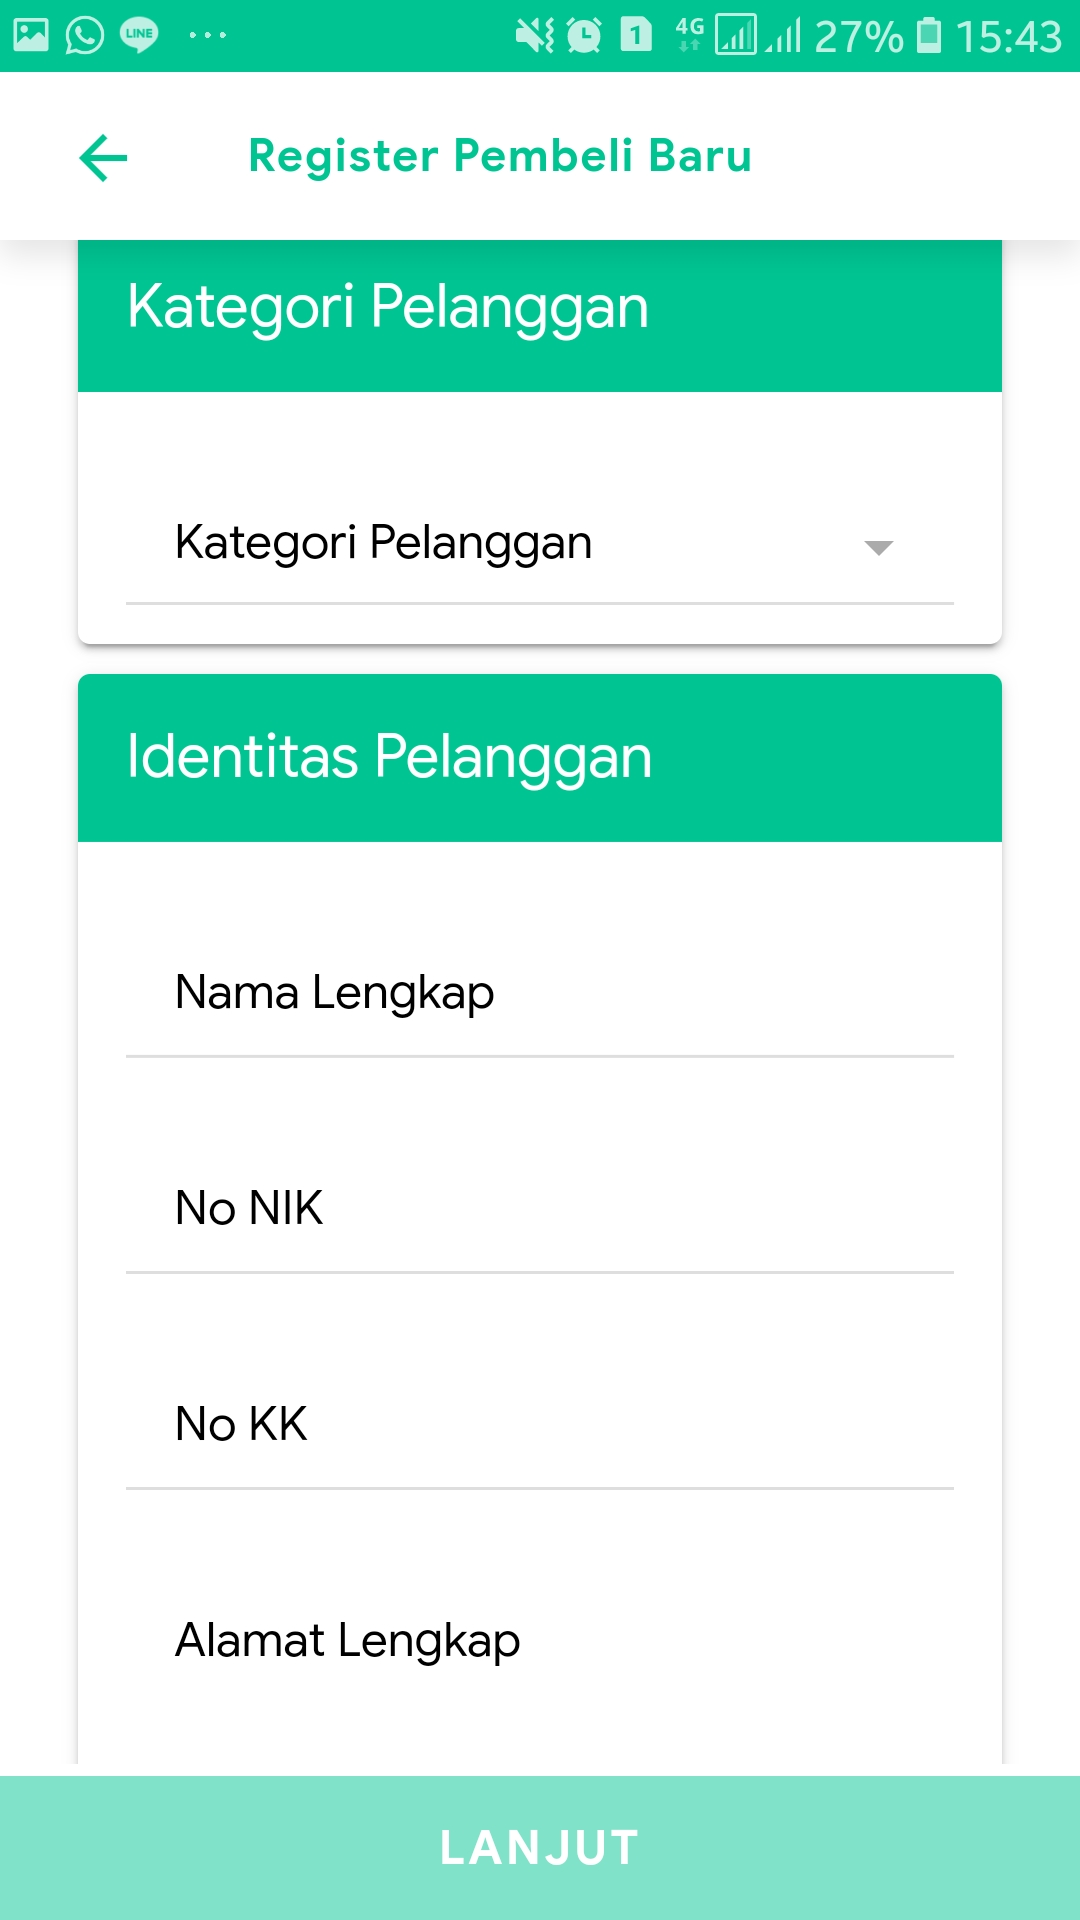
\includegraphics [width = 6cm]{gambar/android/register}
		\caption{Tampilan Halaman Register Pelanggan}
		\label{tampilanRegisterPangkalan}
	\end{figure}

	\begin{figure}[H]
		\center
		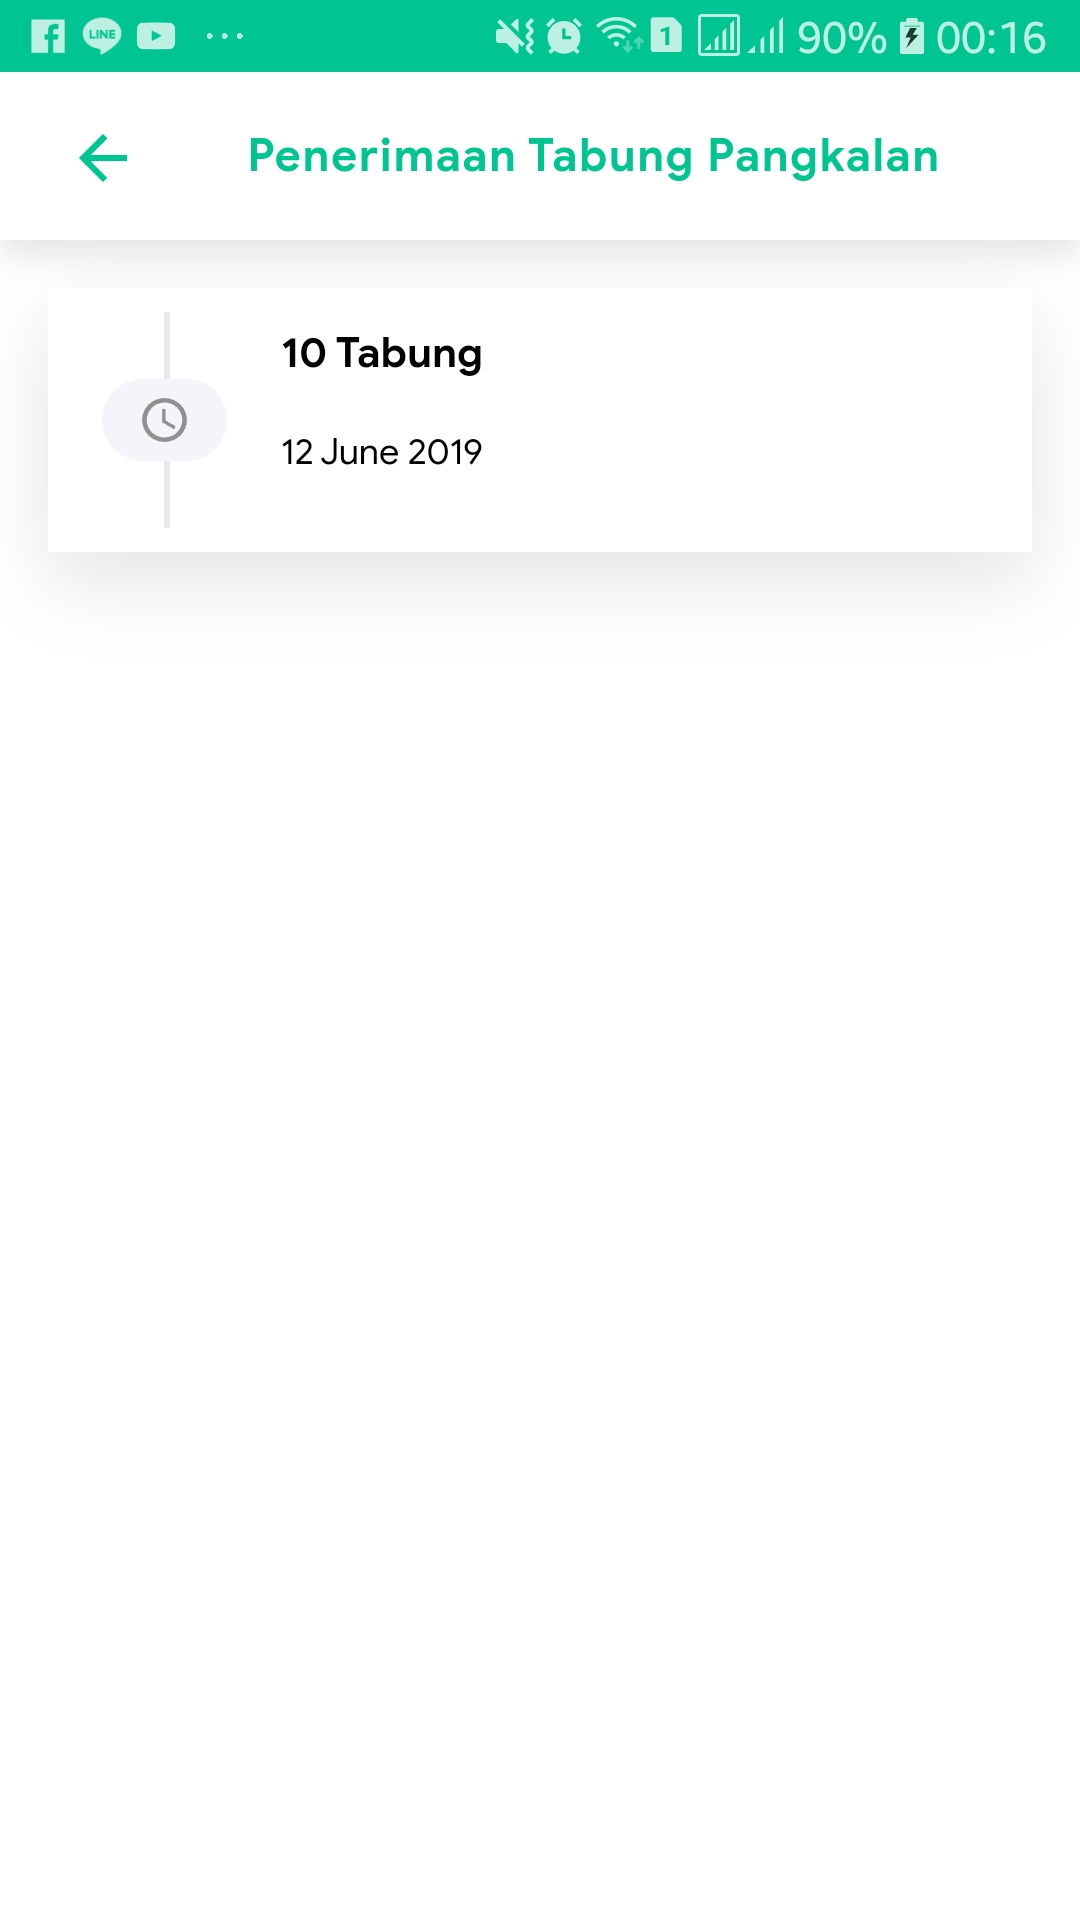
\includegraphics [width = 6cm]{gambar/android/penerimaan}
		\caption{Tampilan Halaman Penerimaan Pasokan Tabung}
		\label{tampilanPenerimaanPangkalan}
	\end{figure}

	\begin{figure}[H]
		\center
		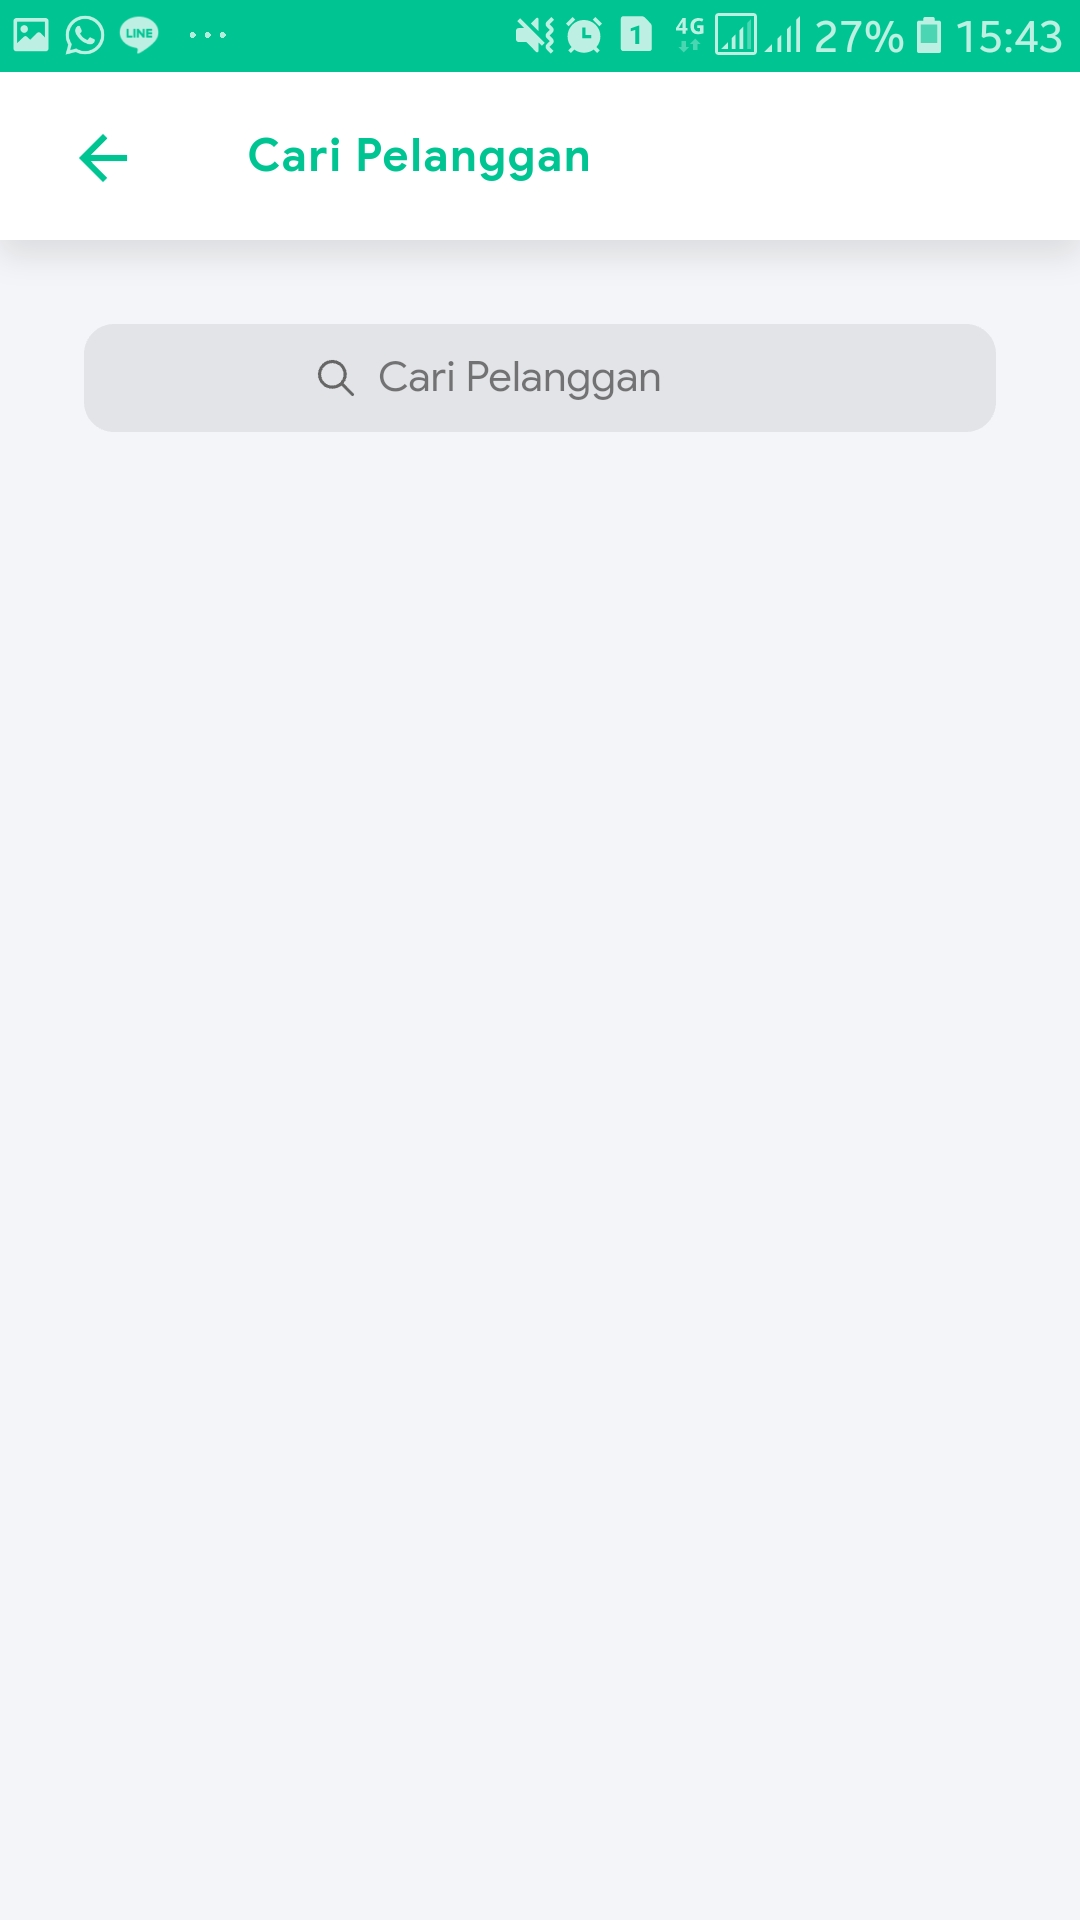
\includegraphics [width = 6cm]{gambar/android/cari-pelanggan}
		\vspace{1cm}
		\hspace{1cm}
		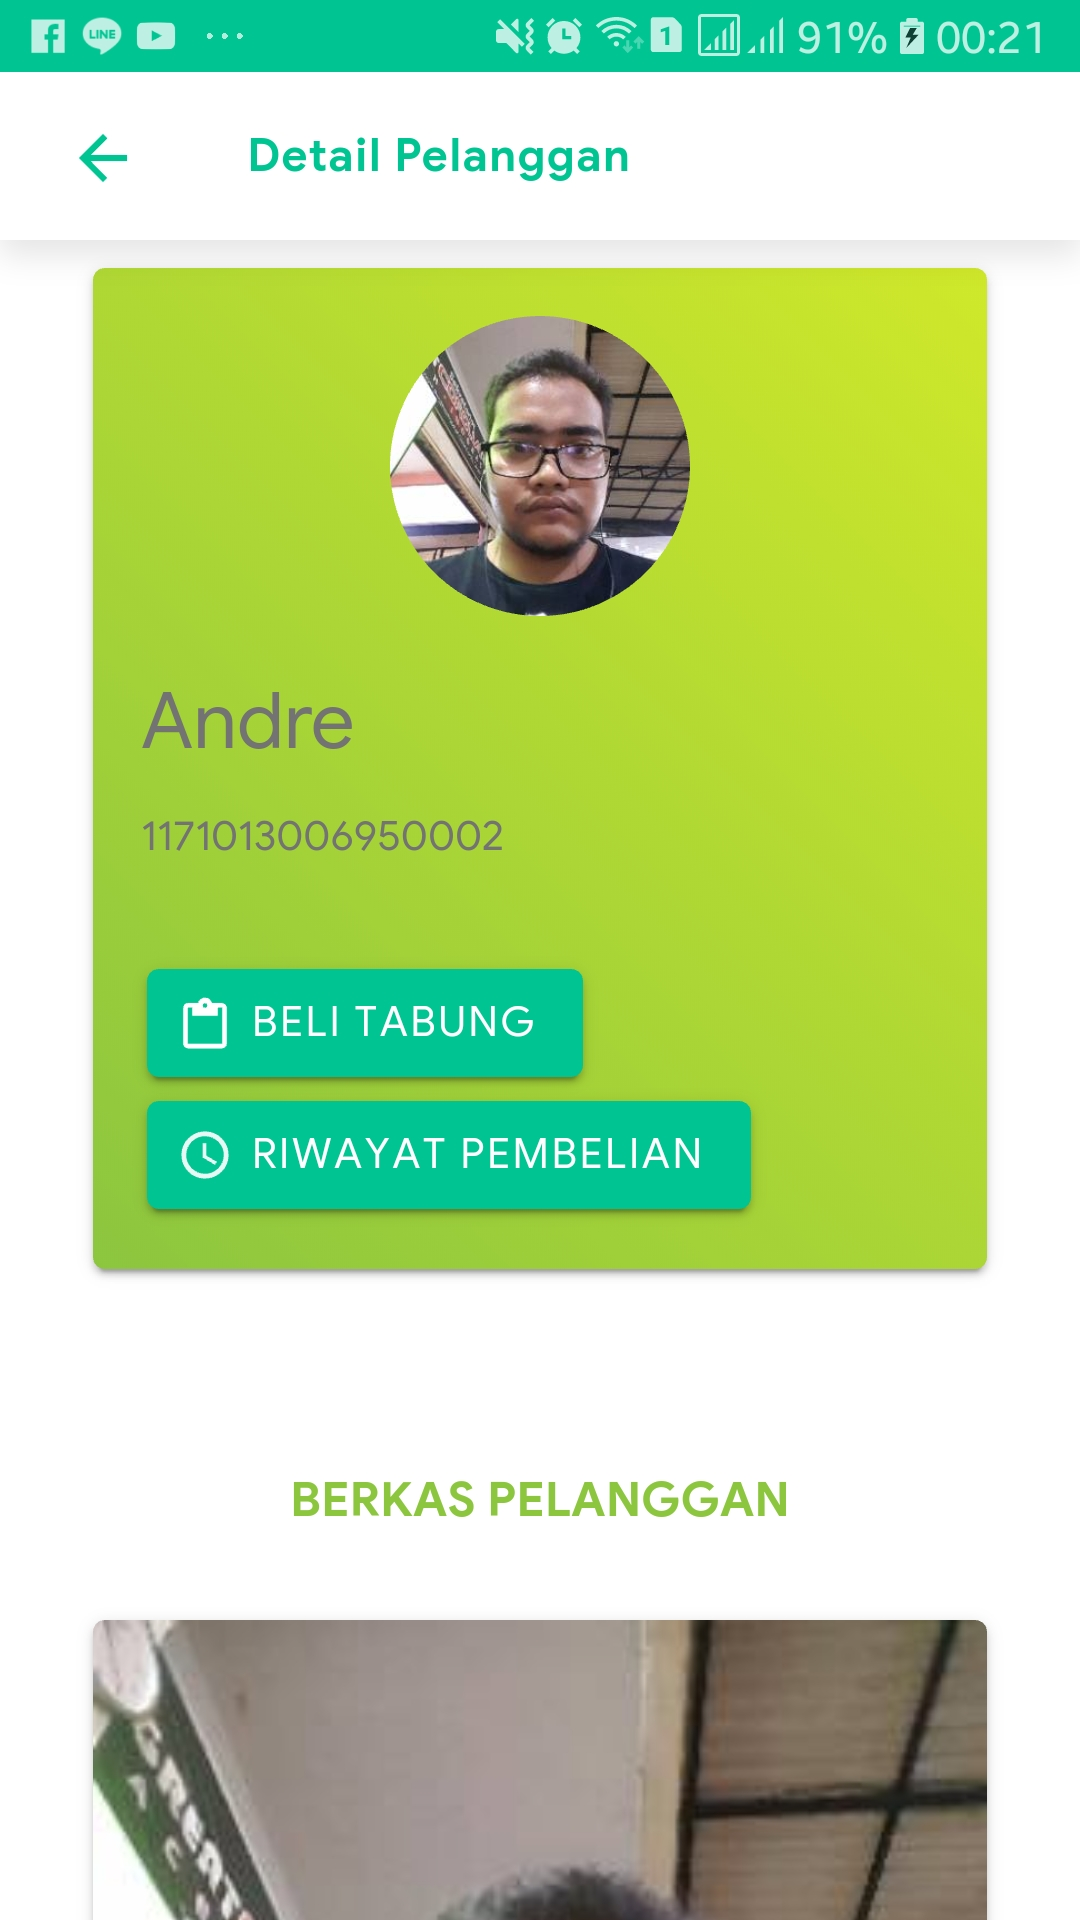
\includegraphics [width = 6cm]{gambar/android/detail-pelanggan}
		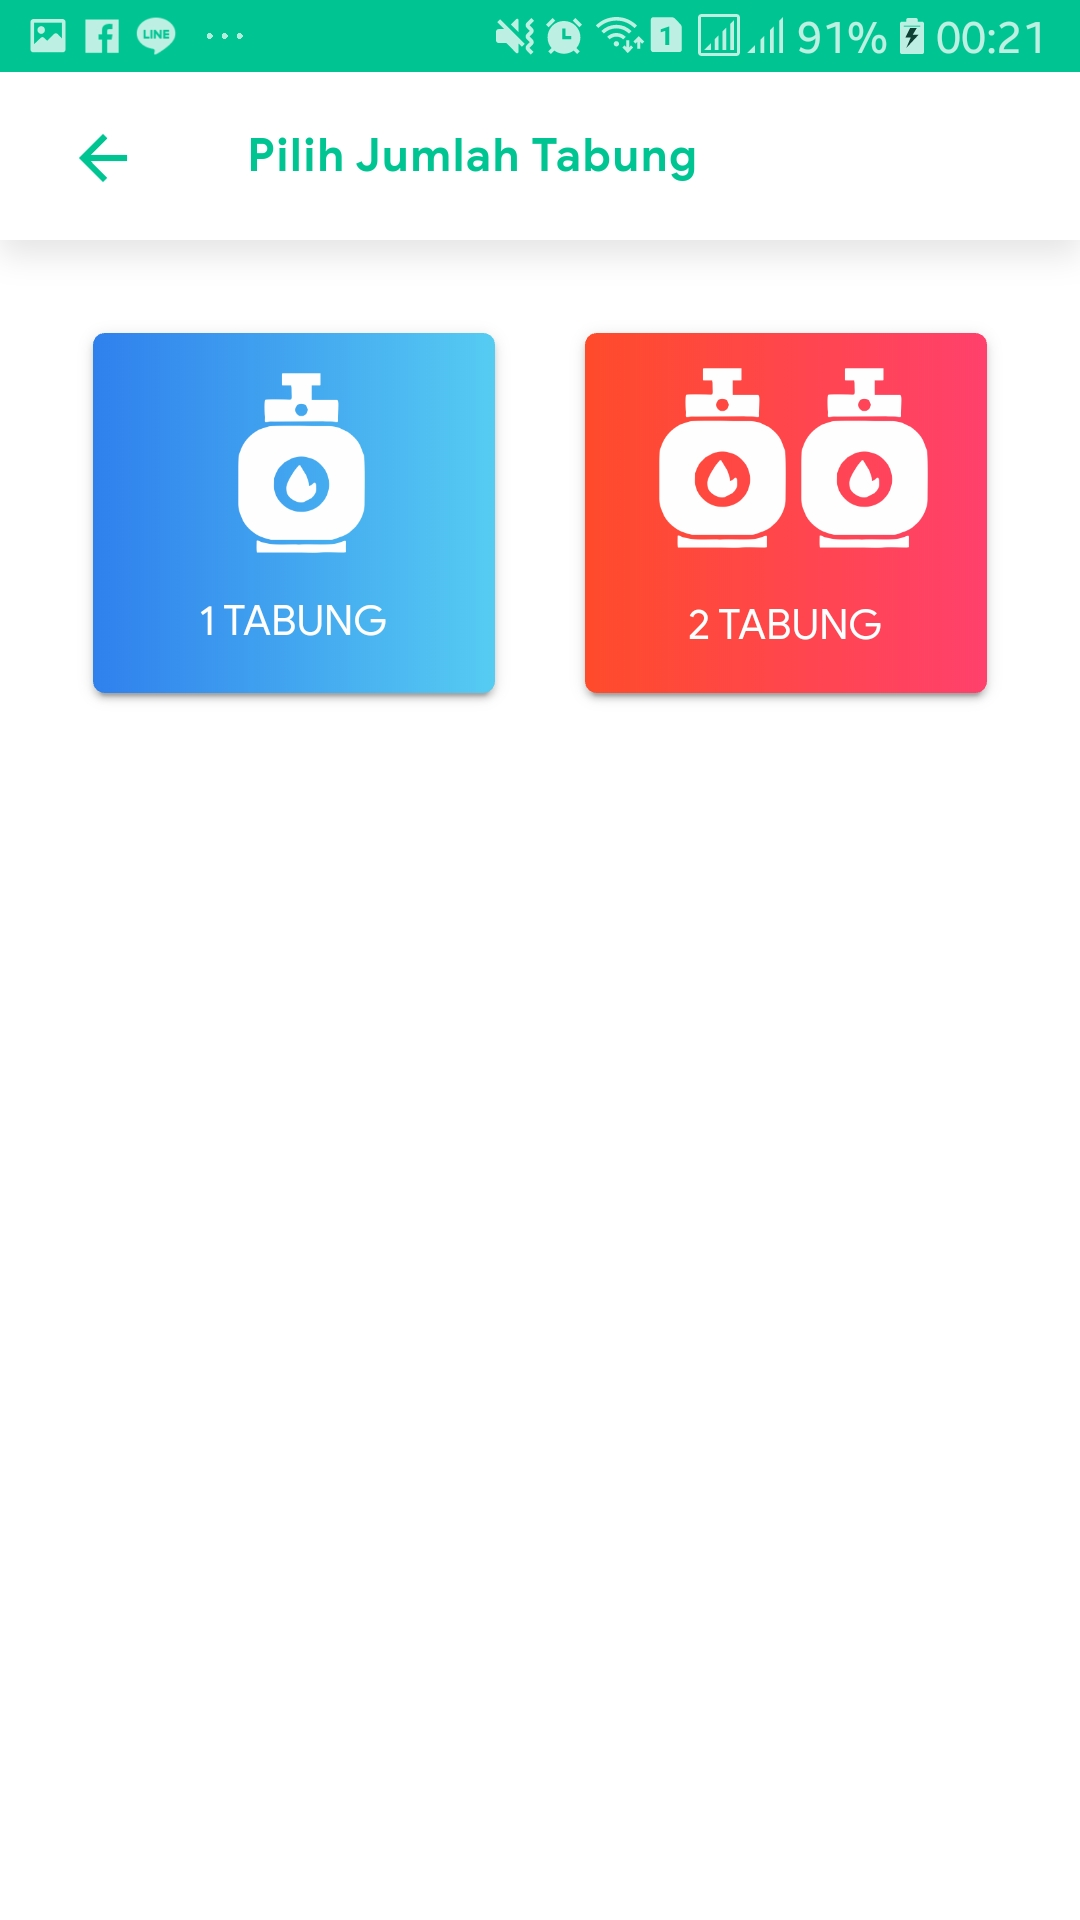
\includegraphics [width = 6cm]{gambar/android/pilih-tabung}
		\hspace{1cm}
		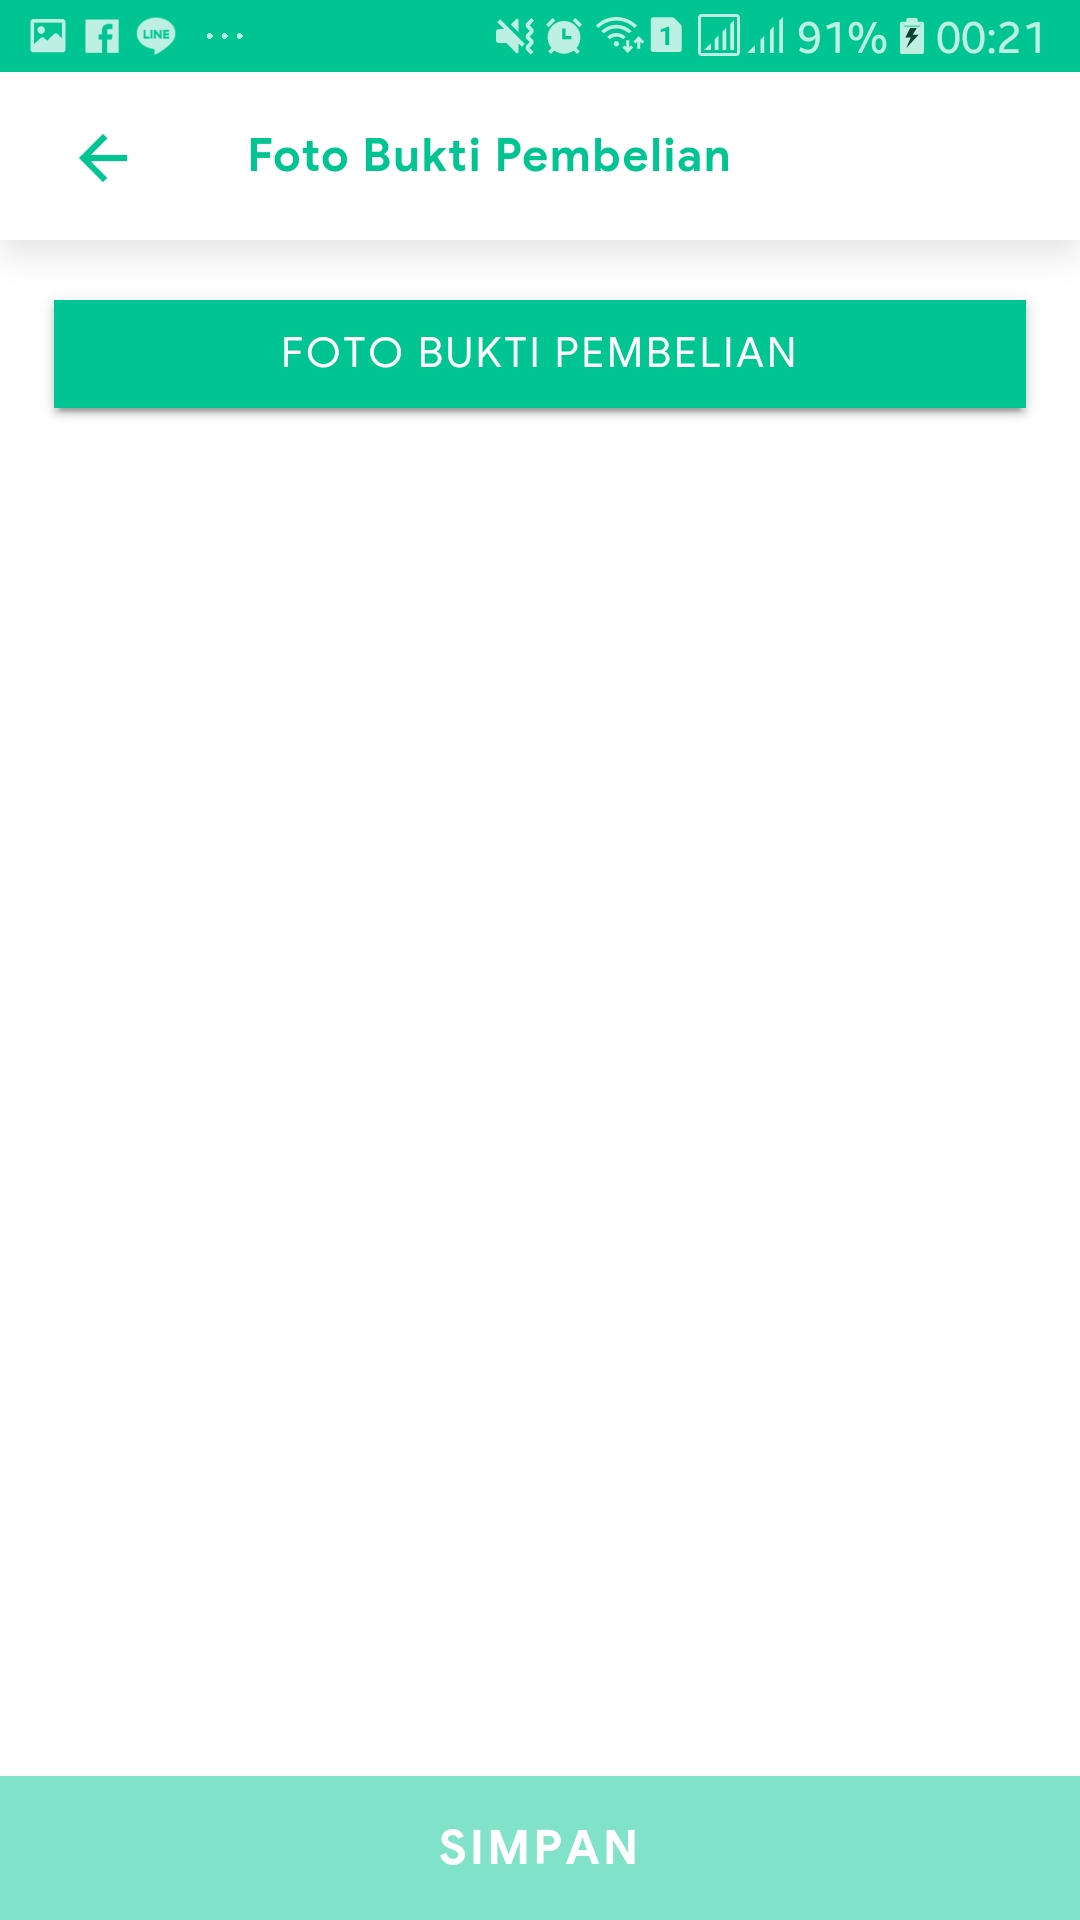
\includegraphics [width = 6cm]{gambar/android/bukti-pembelian}
		\caption{Tampilan Halaman Pembelian Tabung}
		\label{tampilanPembelianPangkalan}
	\end{figure}

	\par Tampilan Aplikasi berbasis web untuk agen gas LPG 3Kg ini terdiri dari 5 halaman utama yaitu halaman beranda, halaman pangkalan, halaman rencana pasokan tabung, halaman pembeli, dan halaman untuk melakukan ekspor laporan penyaluran.
	\par Sebelumnya masuk ke dalam aplikasi ini, agen harus melakukan login menggunakan email khususnya email google seperti pada Gambar \ref{tampilanLoginAgen}. Setelah berhasil melakukan login maka akan ditujukan ke halaman beranda, pada halaman ini terdapat status jumlah pangkalan, jumlah penjualan rata-rata bulan ini dan tahun ini seperti pada \ref{tampilanBerandaAgen}.
	\par Halaman pangkalan berfungsi untuk menampilkan daftar pangkalan pada agen tersebut, disini agen dapat melakukan penambahan dengan menekan tombol "tambah pangkalan"dan perubahan pada data pangkalan dengan menekan tombol "profil" seperti pada Gambar \ref{tampilanDaftarPangkalanAgen}. Pada halaman ini juga memiliki aksi untuk membuat rencana pasokan tabung untuk pangkalan dengan menekan tombol "rencana pasokan" yang akan ditujukan ke halaman daftar rencana pasokan tabung untuk pangkalan tersebut seperti pada Gambar \ref{tampilanPenerimaanAgen}. Halaman rencana pasokan ini berfungsi untuk menginput data rencana pasokan untuk bulan depan. Data-data ini nantinya harus di verifikasi oleh pangkalan via aplikasi berbasis android sehingga datanya akan tersinkronisasi.
	\par Halaman laporan berfungsi untuk melakukan ekspor laporan penyaluran ke dalam bentuk PDF seperti pada Gambar \ref{tampilanLaporanAgen}.
	
	\begin{figure}[H]
		\center
		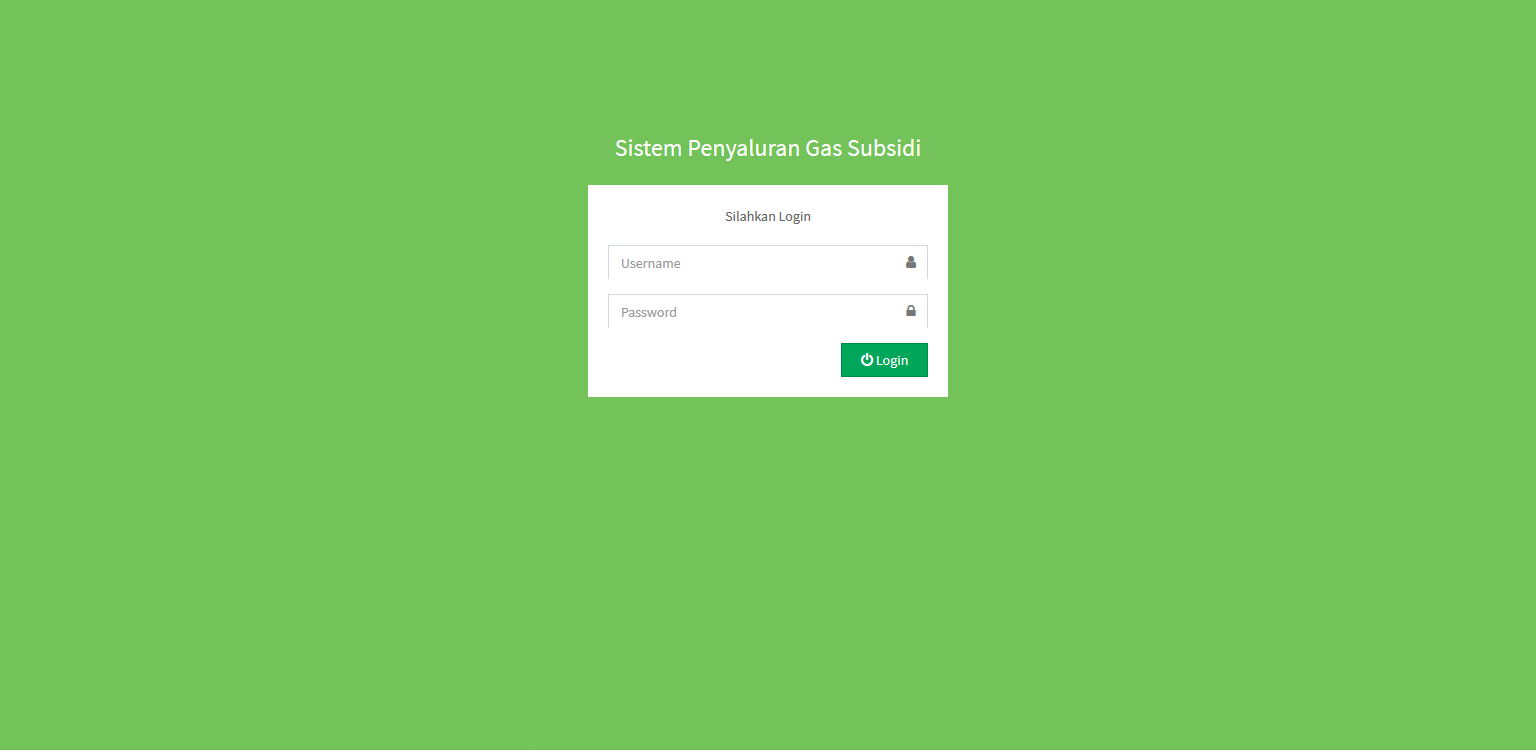
\includegraphics [width = 9cm]{gambar/web/login}
		\caption{Tampilan Halaman Login untuk Agen Gas LPG 3Kg}
		\label{tampilanLoginAgen}
	\end{figure}
	
	\begin{figure}[H]
		\center
		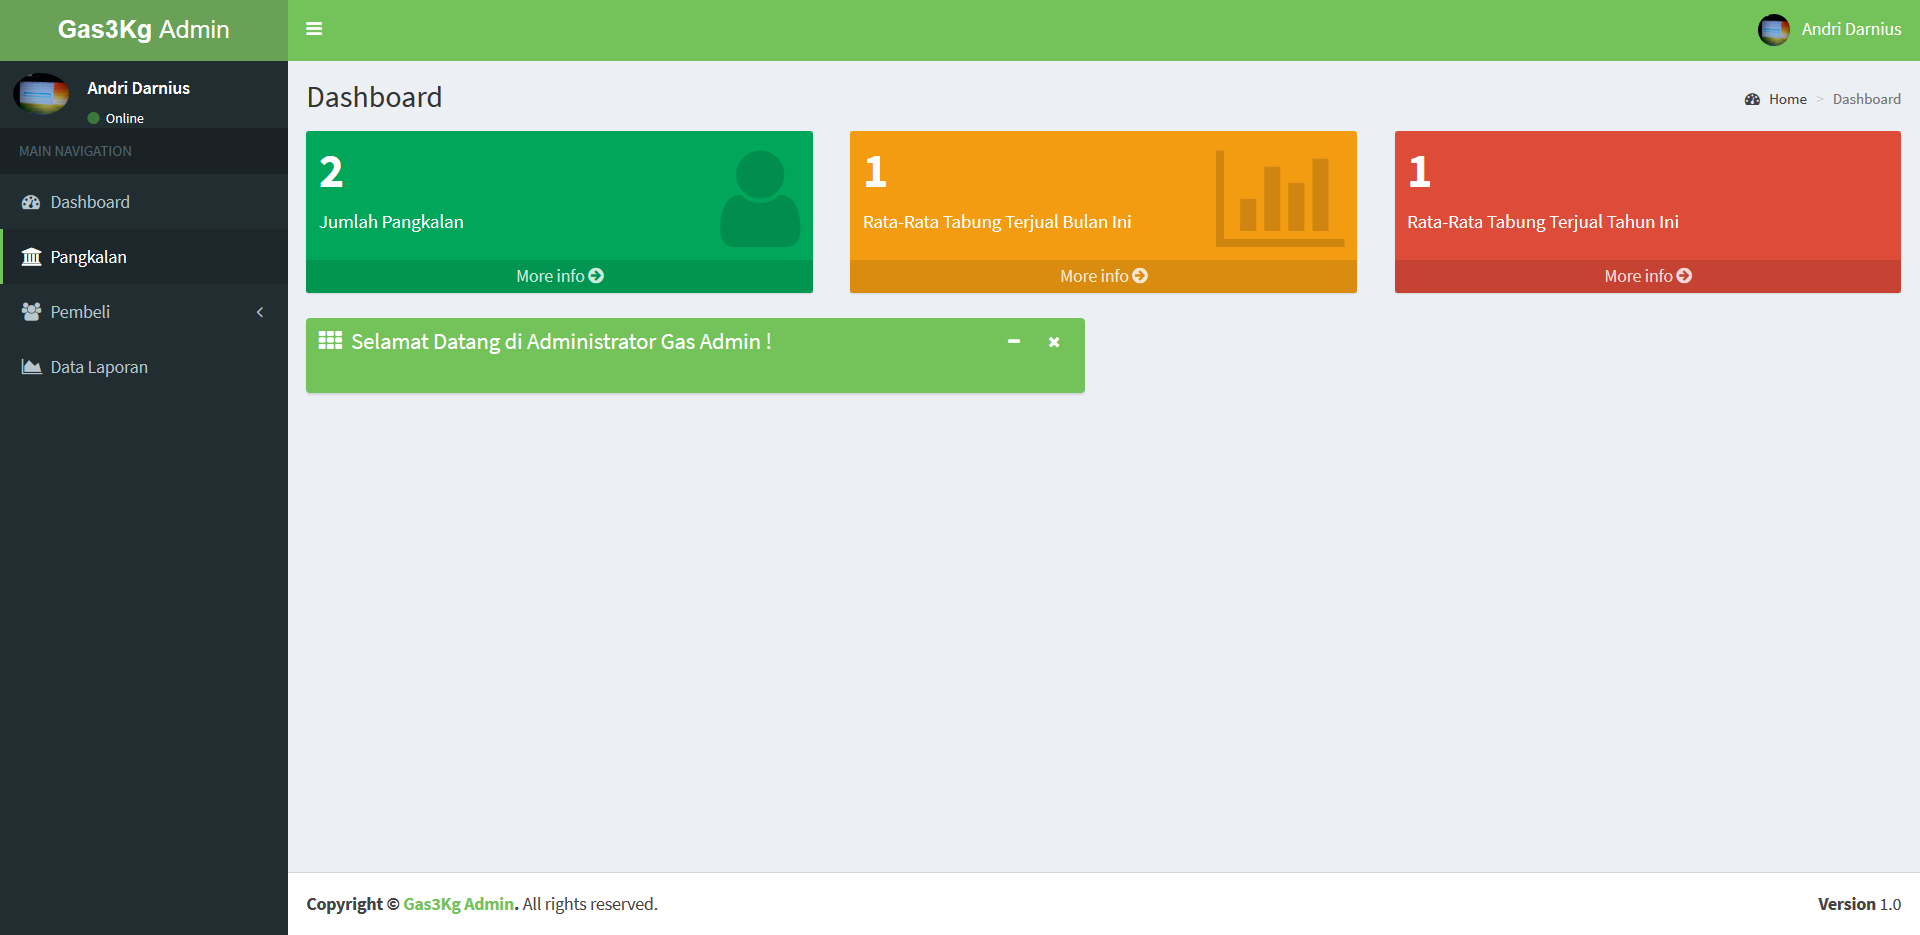
\includegraphics [width = 9cm]{gambar/web/beranda}
		\caption{Tampilan Halaman Beranda untuk Agen Gas LPG 3Kg}
		\label{tampilanBerandaAgen}
	\end{figure}

	\begin{figure}[H]
		\center
		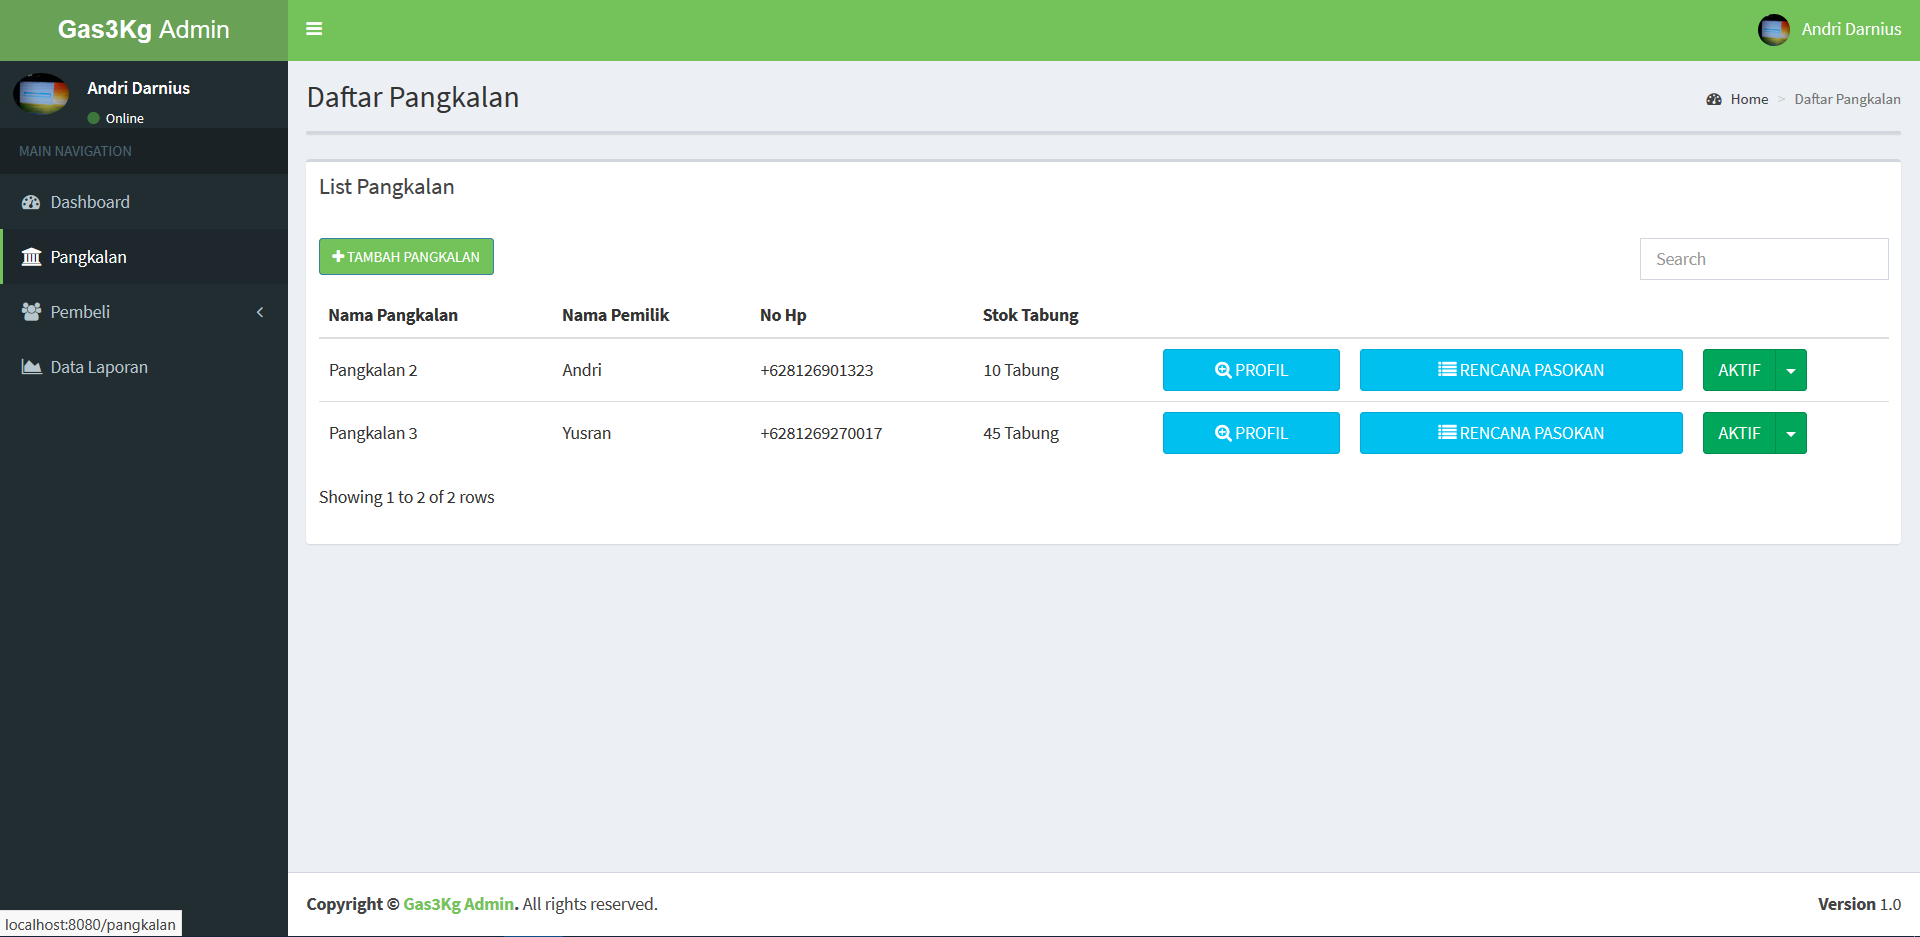
\includegraphics [width = 9cm]{gambar/web/pangkalan}
		\caption{Tampilan Halaman Daftar Pangkalan }
		\label{tampilanDaftarPangkalanAgen}
	\end{figure}

	\begin{figure}[H]
		\center
		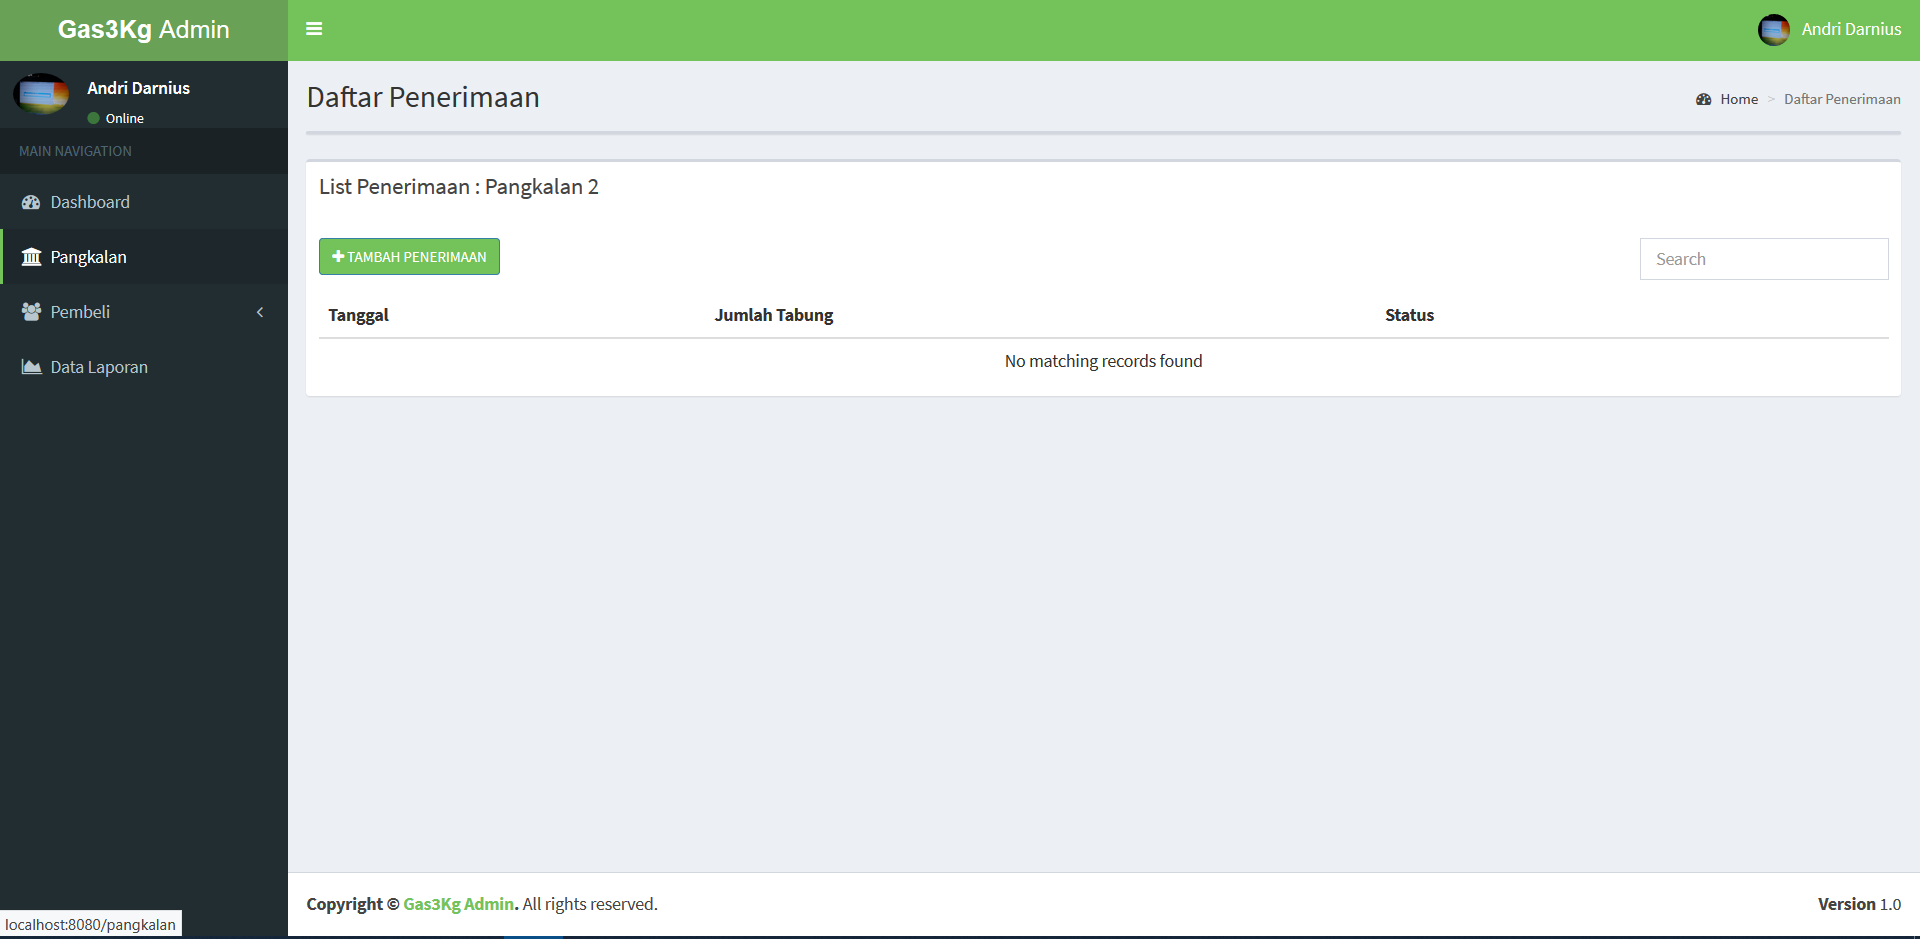
\includegraphics [width = 9cm]{gambar/web/penerimaan}
		\caption{Tampilan Halaman Rencana Penerimaan Pasokan Tabung}
		\label{tampilanPenerimaanAgen}
	\end{figure}

	\begin{figure}[H]
		\center
		\includegraphics [width = 9cm]{gambar/web/Laporan}
		\caption{Tampilan Halaman Ekspor Laporan}
		\label{tampilanLaporanAgen}
	\end{figure}
	
	
	
	\subsection{Pembuatan Sistem}
	
	\begin{enumerate}[a.]
		\item Layanan Web
		\\ Layanan web dikembangkan menggunakan bahasa pemrograman java dengan memanfaatkan pustaka Google Endpoints API untuk membangun sebuah layanan web yang memiliki prinsip RESTful API. dan juga menggunakan Google Datastore sebagai media penyimpanan basis data. Google Datastore merupakan layanan basis data NoSQL yang dibuat untuk penskalaan otomatis, kinerja tinggi, dan kemudahan dalam pengembangan aplikasi. Dikarenakan kita menggunakan Google Datastore sebagai Layanan penyimpanan basis data, kita akan menggunakan salah satu pustaka Java yang dimilikinya yaitu Objectify. Pada pembuatan layanan web (\textit{webservice}) hanya membutuhkan \textit{Model} Basis Data, \textit{Controller}, dan API. Pada pembuatan \textit{Model} basis data, desain basis datanya akan mengikuti dari desain \textit{class diagram} yang dibuat sebelumnya. tahap pembuatan layanan web yang pertama adalah membuat kelas \textit{Model} untuk masing-masing entitas seperti pada Gambar \ref{modelWebservice}. Setelah itu membuat kelas \textit{controller} yang akan menangani setiap operasi untuk memanipulasi data didalam \textit{Model} seperti pada Gambar \ref{controllerWebservice}. Tahap selanjutnya adalah membuat kelas API yang akan menangani pemanggilan setiap \textit{endpoint} yang layanan web seperti pada Gambar \ref{apiWebservice}. Setelah semua komponen telah selesai, maka akan dilakukan pengujian terhadap layanan web untuk mengetahui apakah setiap endpoint berjalan dengan seharusnya seperti pada Gambar \ref{pengujianApi}.
		
		\vspace{-0.4cm}
		\begin{figure}[H]
			\center
			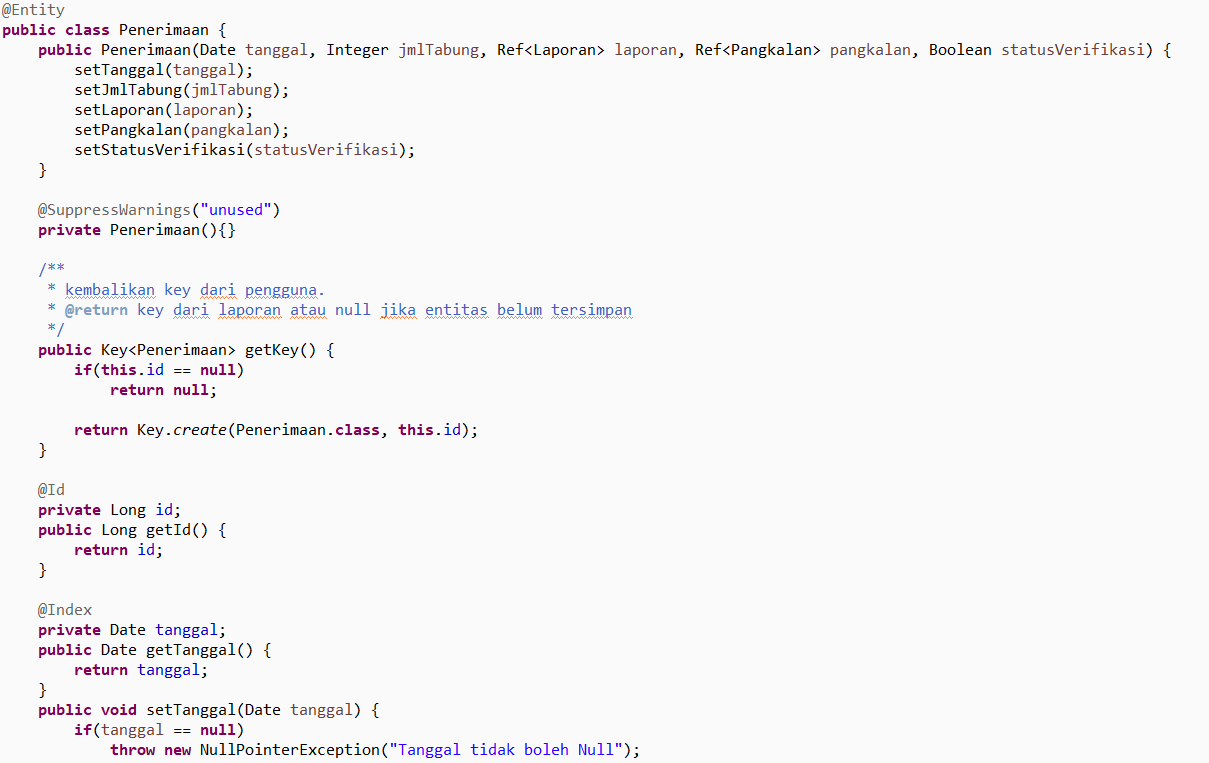
\includegraphics [width = 12cm]{gambar/kode/model-webservice}
			\caption{Potongan kode \textit{model} basis data layanan web}
			\label{modelWebservice}
		\end{figure}
	
		\begin{figure}[H]
			\center
			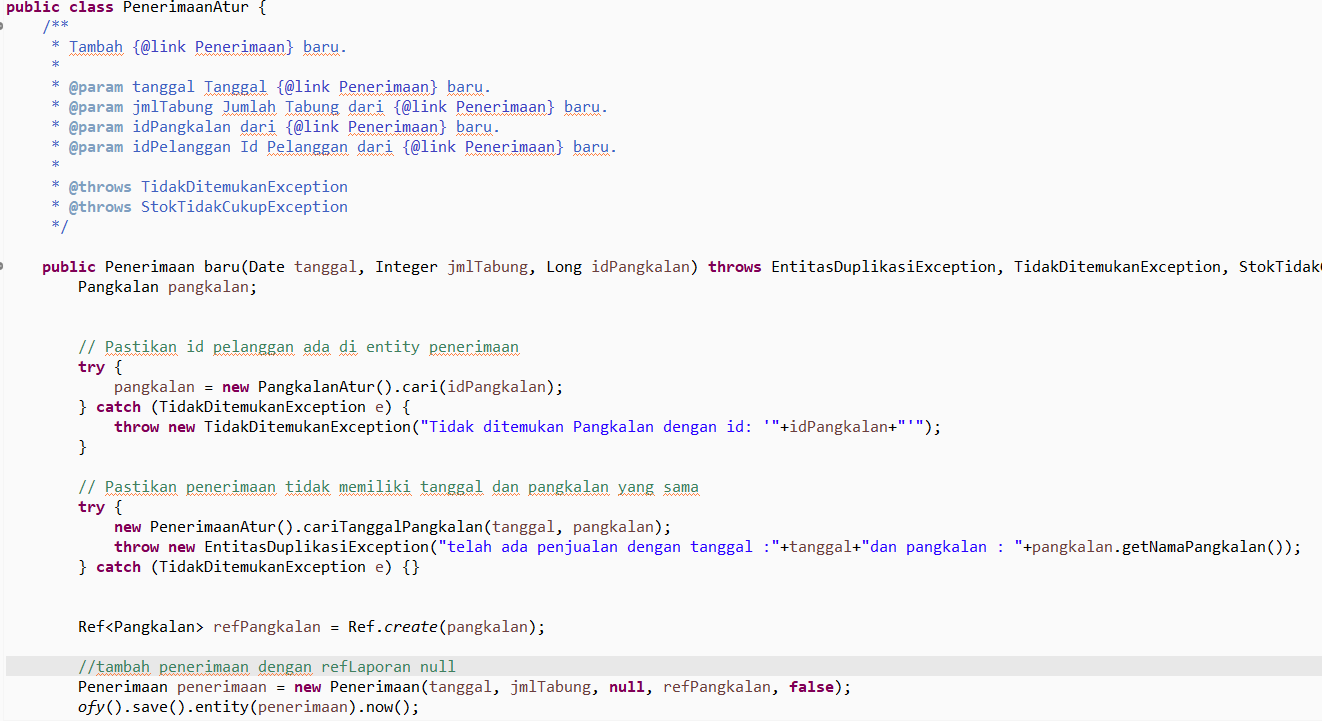
\includegraphics [width = 12cm]{gambar/kode/controller-webservice}
			\caption{Potongan kode \textit{controller} layanan web}
			\label{controllerWebservice}
		\end{figure}
	
		\begin{figure}[H]
			\center
			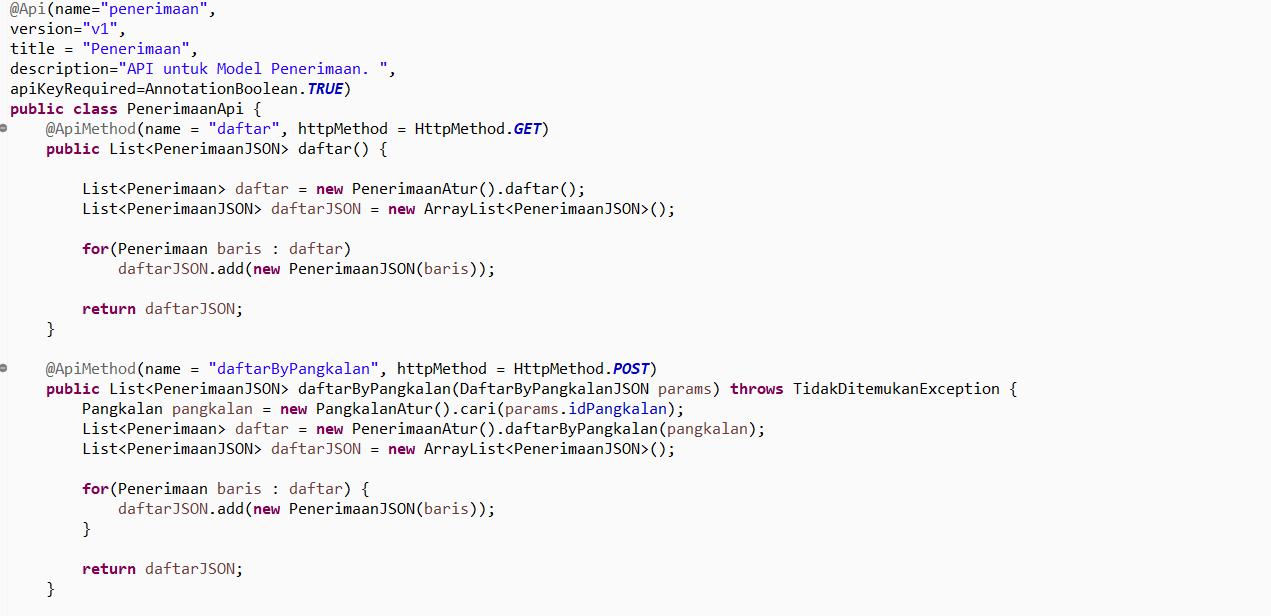
\includegraphics [width = 12cm]{gambar/kode/api-webservice}
			\caption{Potongan kode API layanan web}
			\label{apiWebservice}
		\end{figure}
	
		\begin{figure}[H]
			\center
			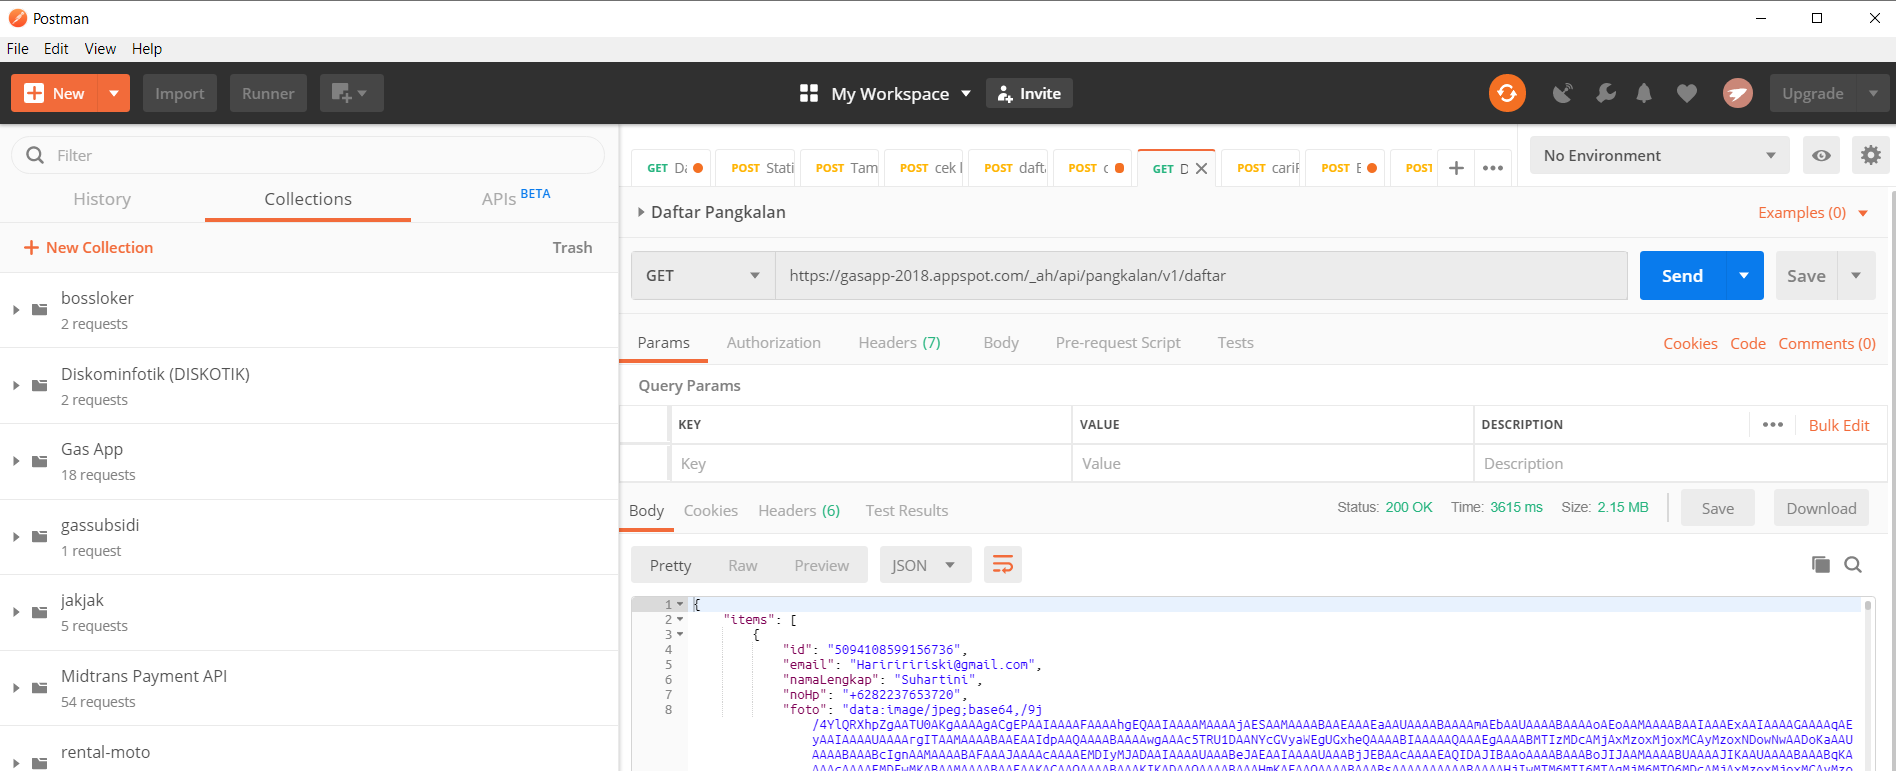
\includegraphics [width = 12cm]{gambar/pengujianApi}
			\caption{Contoh Pengujian Endpoint API pada layanan web (\textit{Webservice})}
			\label{pengujianApi}
		\end{figure} 
		
		\item Aplikasi Mobile
		\\ Aplikasi berbasis \textit{android} dikembangkan menggunakan Ionic Framework yang menggunakan teknologi HTML, JavaScript dan CSS sebagai tampilan \textit{frontend} aplikasi. Pengembangan aplikasi ini mengikuti salah satu prinsip pembuatan aplikasi secara umum yaitu MVC (Model View Controller). Model (providers) berisi fungsi untuk masing-masing method HTTP yang dipanggil oleh aplikasi dari layanan web. \textit{Model} dibuat menggunakan Typescript. \textit{Model} berperan penting pada proses penarikan dan penginputan data ke Google Datastore. Contoh Kode model pada ionic dapat dilihat pada Gambar \ref{modelMobile}. \textit{View} berfungsi untuk mengatur tampilan aplikasi yang ditampilkan pada pengguna melalui HTML dan CSS. Contoh Kode view pada ionic dapat dilihat pada Gambar \ref{modelView}. \textit{Controller} untuk mengatur halaman yang ditampilkan kepada pengguna dan pemanggilan API. \\
		
		\vspace{-0.4cm}
		\begin{figure}[H]
			\center
			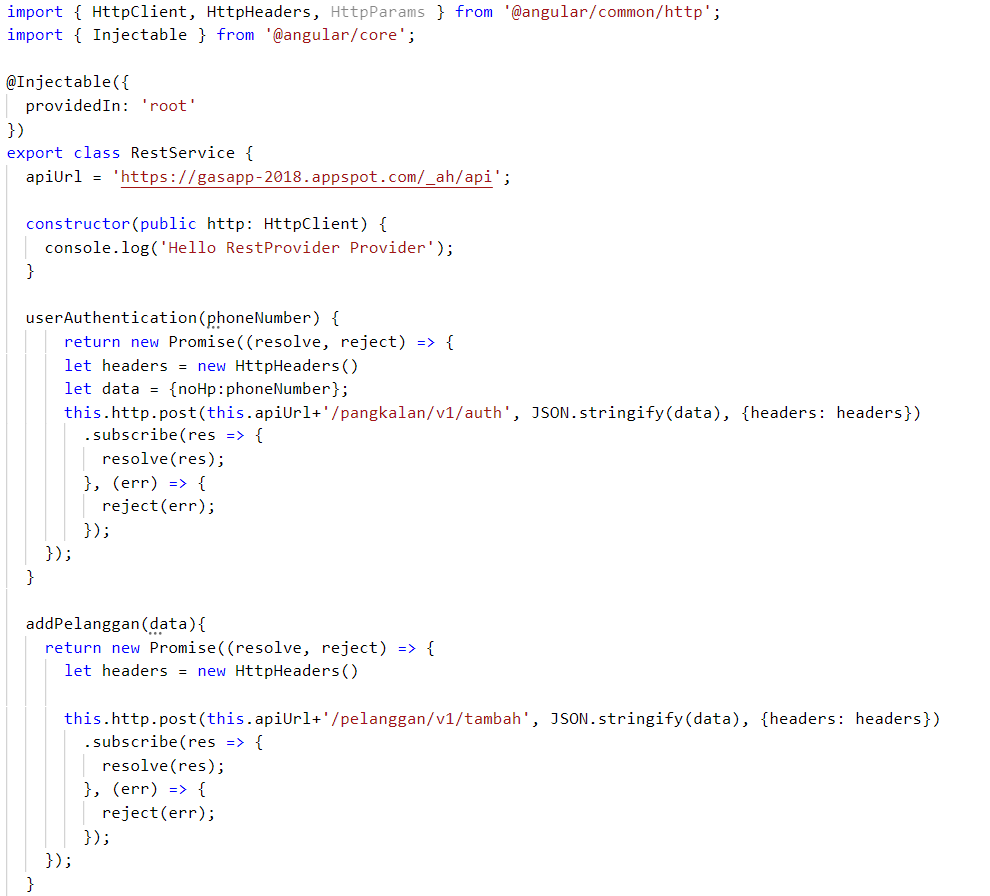
\includegraphics [width = 12cm]{gambar/kode/model-mobile}
			\caption{Potongan kode \textit{model} aplikasi berbasis android}
			\label{modelMobile}
		\end{figure}
		
		\begin{figure}[H]
			\center
			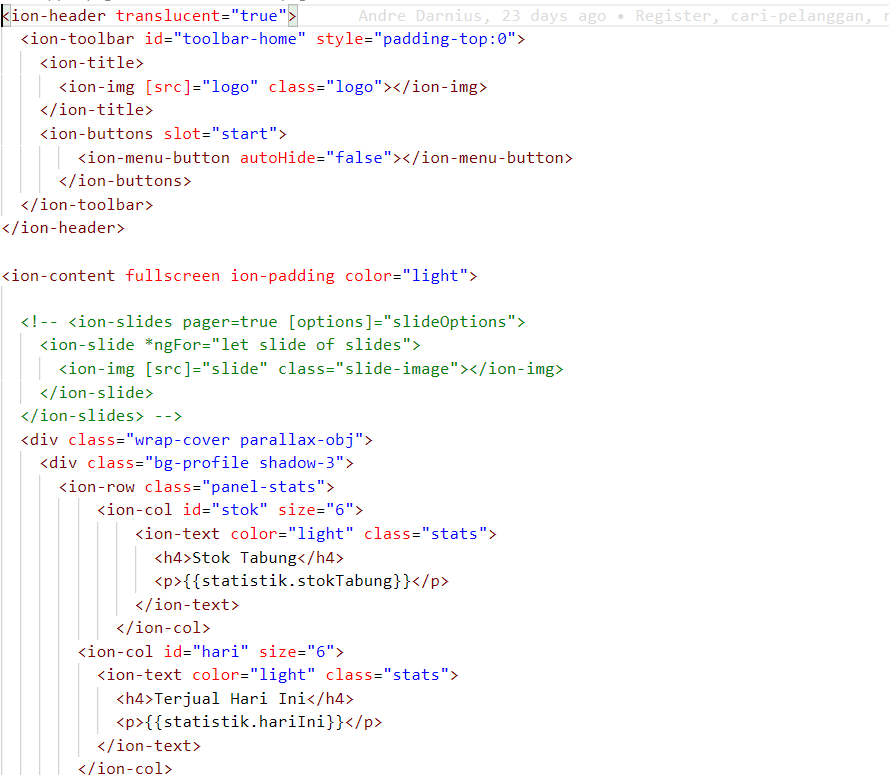
\includegraphics [width = 12cm]{gambar/kode/view-mobile}
			\caption{Potongan kode \textit{view} aplikasi berbasis android}
			\label{viewMobile}
		\end{figure}
		
		\begin{figure}[H]
			\center
			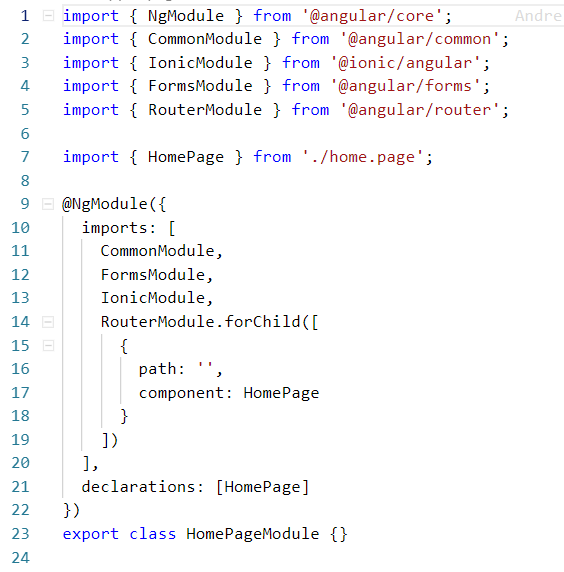
\includegraphics [width = 12cm]{gambar/kode/controller-mobile}
			\caption{Potongan kode \textit{controller} aplikasi berbasis android}
			\label{controllerMobile}
		\end{figure}
		
		 aplikasi ini juga menggunakan layanan Google Firebase untuk dapat melakukan proses login menggunakan nomor HP atau dinamakan dengan \textit{Phone Authentication} seperti pada Gambar \ref{firebaseAuth}
		
		\begin{figure}[H]
			\center
			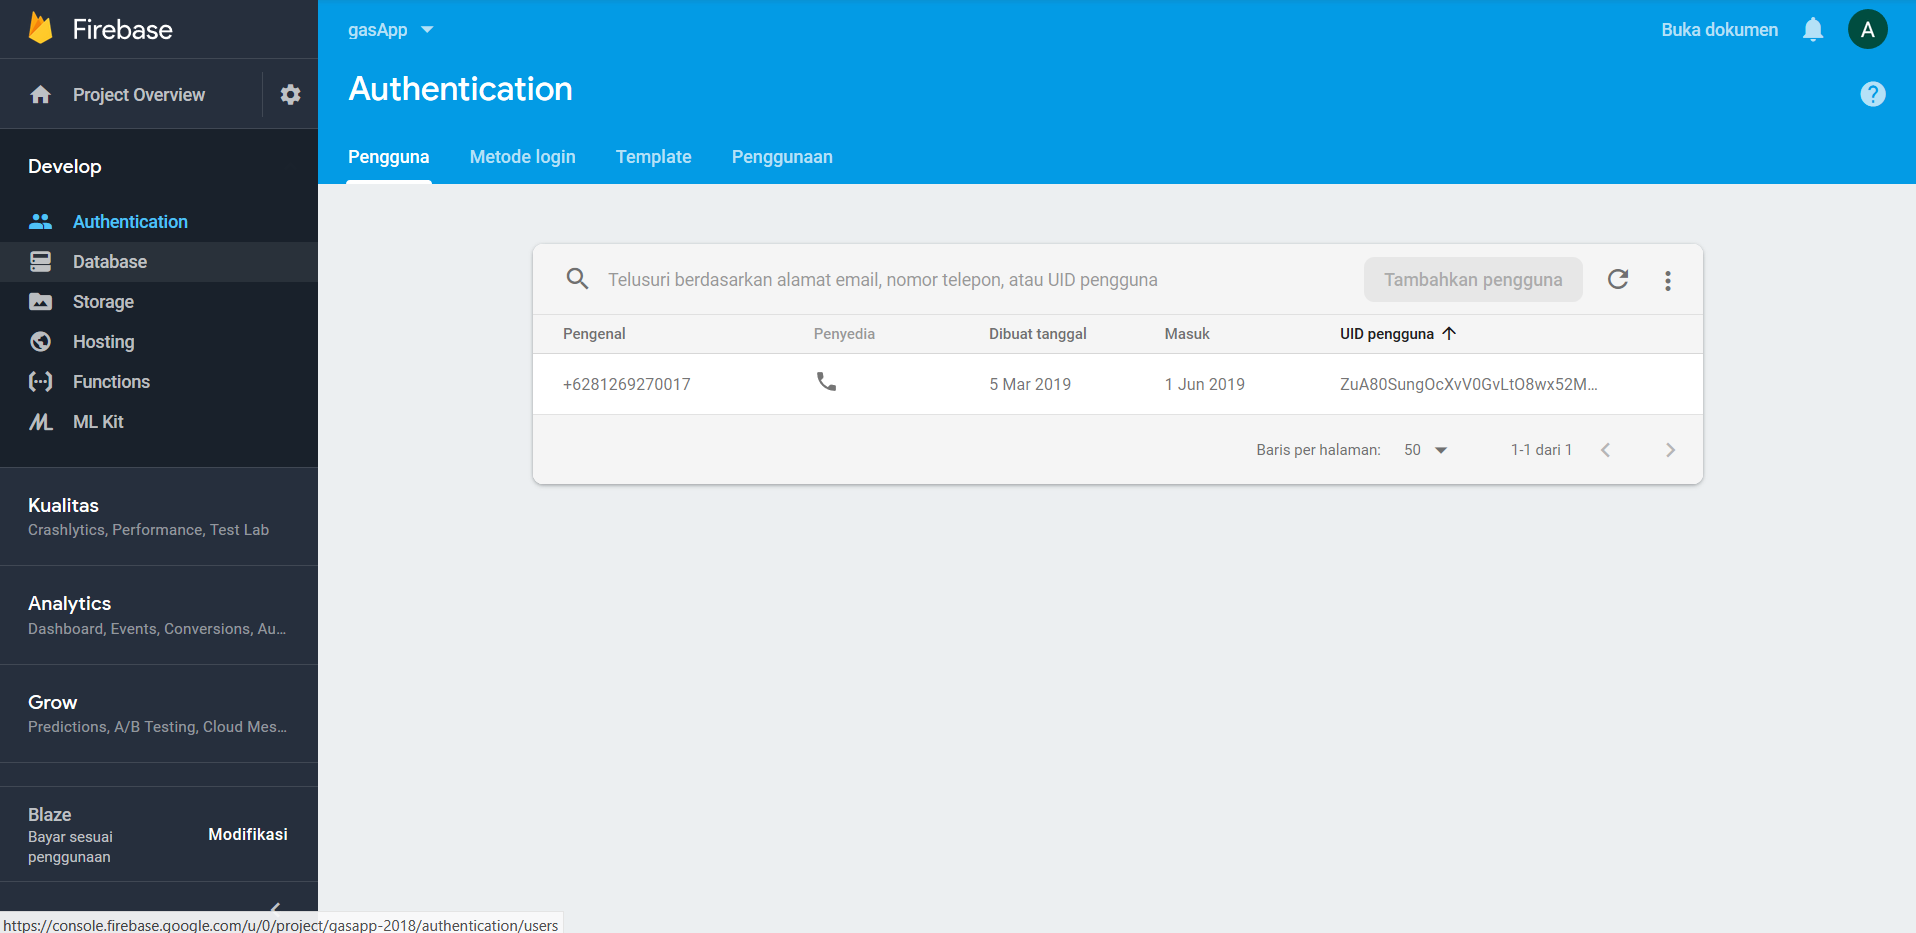
\includegraphics [width = 12cm]{gambar/firebaseAuth}
			\caption{Halaman Konsole  \textit{Phone Authentication} pada Google Firebase}
			\label{firebaseAuth}
		\end{figure} 
	
		\pagebreak
		
		\item Aplikasi Web
		\\ Aplikasi berbasis \textit{web} dikembangkan menggunakan Bahasa pemrograman Java dengan menggunakan prinsip yang sama yaitu MVC (Model View Controller). dimana \textit{model} menggunakan pustaka HTTP untuk memanggil method HTTP pada layanan web dan pustaka GSON untuk melakukan proses konversi dari JSON ke dalam objek java. untuk \textit{view} menggunakan JSP (\textit{Java Server Page}) untuk menampilkan isi halaman \textit{web} yang akan dibangun. JSP memiliki struktur bahasa yang hampir sama dengan HTML (\textit{Hypertext Markup Language}). untuk \textit{controller} menggunakan pustaka HTTP Servlet untuk menangani permintaan HTTP URL dan mengatur pemanggilan \textit{view dan model}. Aplikasi ini nanti akan berjalan pada platform Google App Engine (GAE)\\
		
		\vspace{-0.4cm}
		\begin{figure}[H]
			\center
			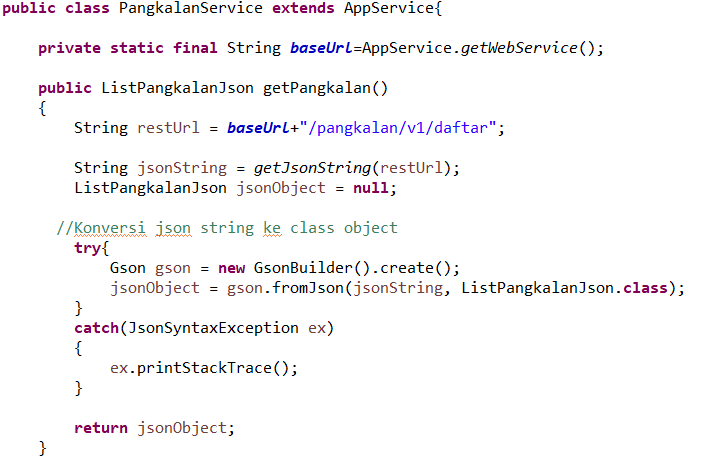
\includegraphics [width = 14cm]{gambar/kode/model-web}
			\caption{Potongan kode \textit{model} aplikasi berbasis web}
			\label{modelWeb}
		\end{figure}
		
		\begin{figure}[H]
			\center
			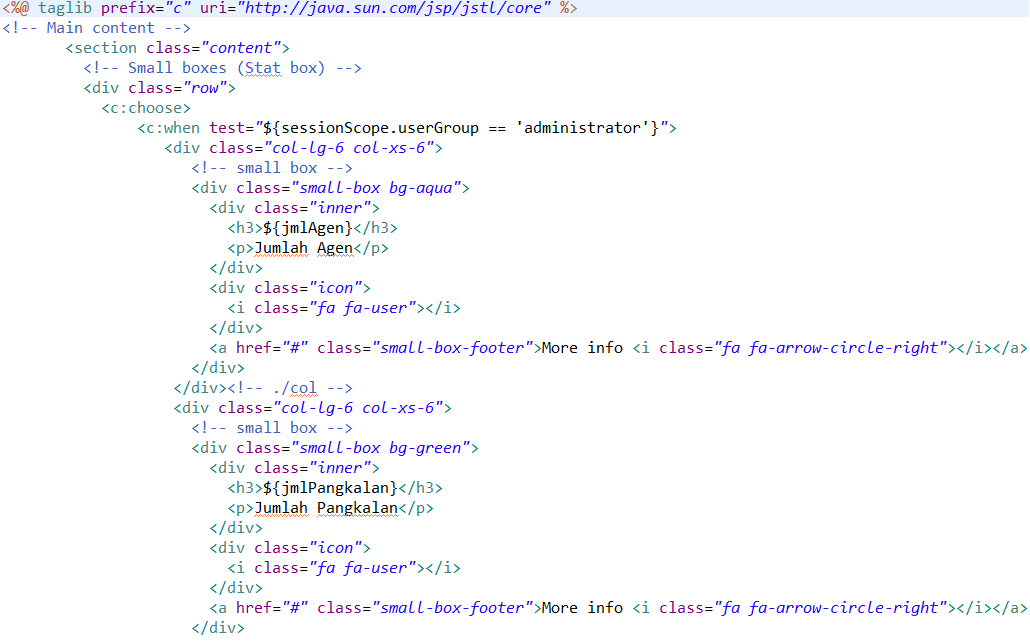
\includegraphics [width = 15cm]{gambar/kode/view-web}
			\caption{Potongan kode \textit{view} aplikasi berbasis web}
			\label{viewWeb}
		\end{figure}
		
		\begin{figure}[H]
			\center
			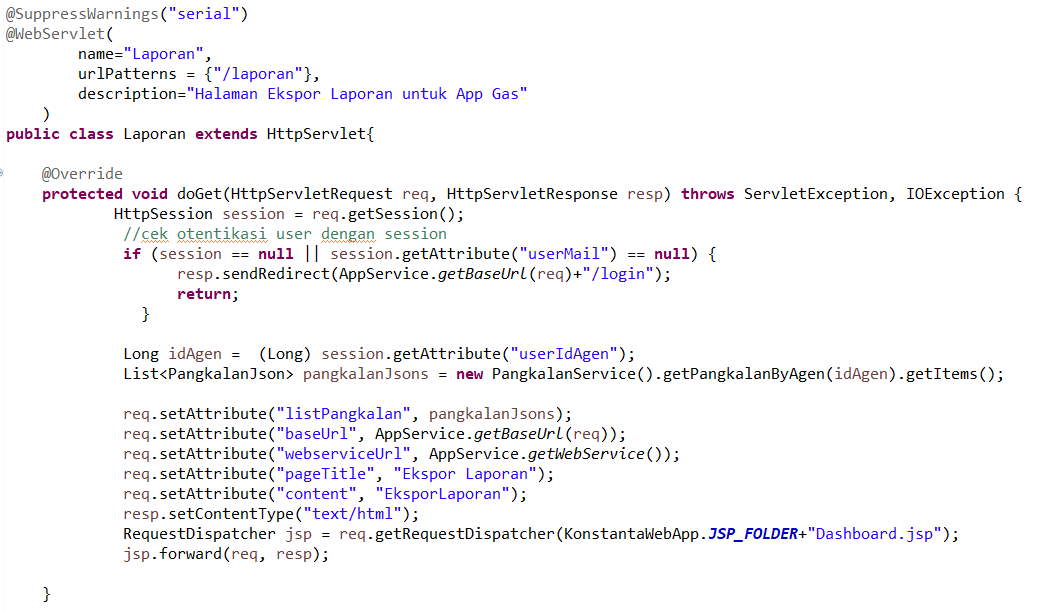
\includegraphics [width = 14cm]{gambar/kode/controller-web}
			\caption{Potongan kode \textit{controller} aplikasi berbasis web}
			\label{controllerWeb}
		\end{figure}
	
		Aplikasi berbasis web ini menggunakan layanan Google Sign-in untuk melakukan proses login dengan memakai email google sebagai ID Pengenal. Untuk proses implementasinya hanya dengan menanamkan \textit{script} javascript pada halaman login seperti pada Gambar \ref{loginWeb}. Aplikasi ini juga memakai pustaka java yang bernama itext untuk melakukan ekspor data penyaluran tabung dalam bentuk \textit{file} PDF. Berikut potongan kode untuk melakukan proses ekspor pada Gambar \ref{eksporWeb}.
	
		\begin{figure}[H]
			\center
			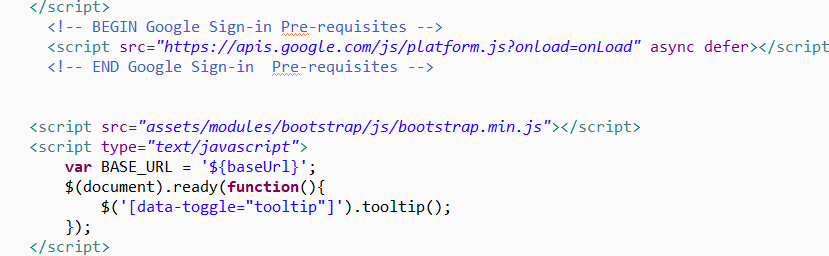
\includegraphics [width = 14cm]{gambar/kode/login-web}
			\caption{Potongan kode Login memakai email aplikasi berbasis web}
			\label{loginWeb}
		\end{figure}
	
		\begin{figure}[H]
			\center
			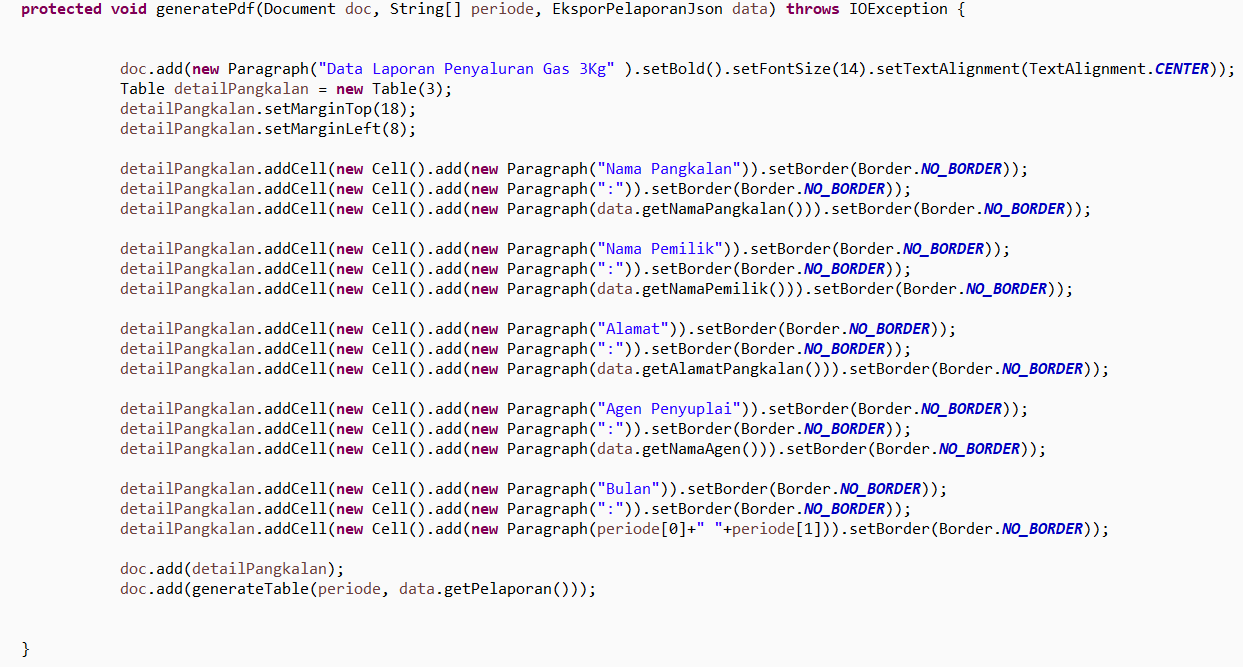
\includegraphics [width = 14cm]{gambar/kode/ekspor-web}
			\caption{Potongan kode ekspor data aplikasi berbasis web}
			\label{eksporWeb}
		\end{figure}

	\end{enumerate}

	
	\section{Pengujian Sistem}
	
		\subsection{Metode \textit{Whitebox}}
			\par Pada pengujian \textit{whitebox}, aplikasi ini menggunakan JUnit yang dapat melakukan pengujian secara otomatis. Aspek-aspek yang diuji pada pengujian ini adalah bagaimana program yang dibangun bukan hanya dapat berjalan dengan semestinya (\textit{test success}), tapi pada saat diberikan sebuah parameter yang salah program dapat mengembalikan error yang semestinya (\textit{test fail}). Aplikasi yang dibangun telah dianggap lulus pengujian apabila mampu melewati semua \textit{test} secara sempurna 100\%. 
			
			\begin{figure}[H]
				\center
				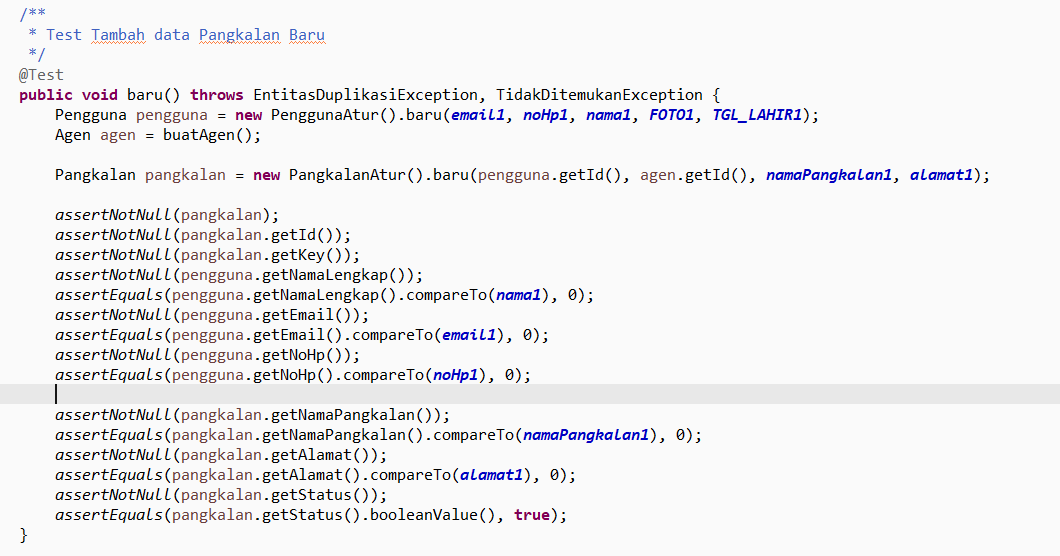
\includegraphics [width = 14cm]{gambar/kode/test-success}
				\caption{Potongan kode Pengujian JUnit dengan kasus berhasil (\textit{test success})}
				\label{testSuccess}
			\end{figure}
		
			\begin{figure}[H]
				\center
				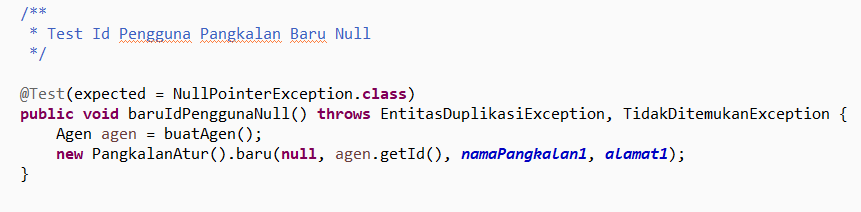
\includegraphics [width = 14cm]{gambar/kode/test-fail}
				\caption{Potongan kode Pengujian JUnit dengan kasus gagal (\textit{test fail})}
				\label{testFail}
			\end{figure}
		
			\begin{figure}[H]
				\center
				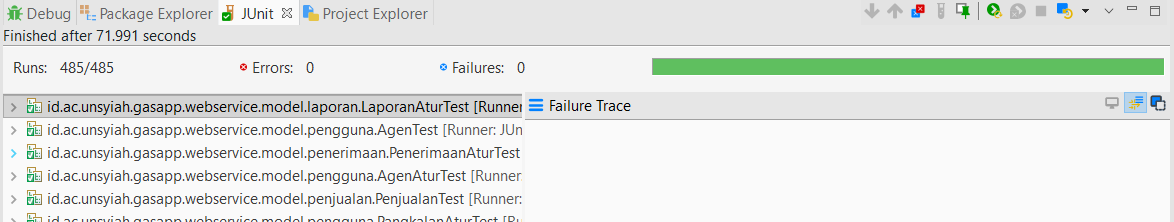
\includegraphics [width = 14cm]{gambar/kode/junit-success}
				\caption{Pengujian JUnit Berhasil}
				\label{junitSuccess}
			\end{figure}
		
			\begin{figure}[H]
				\center
				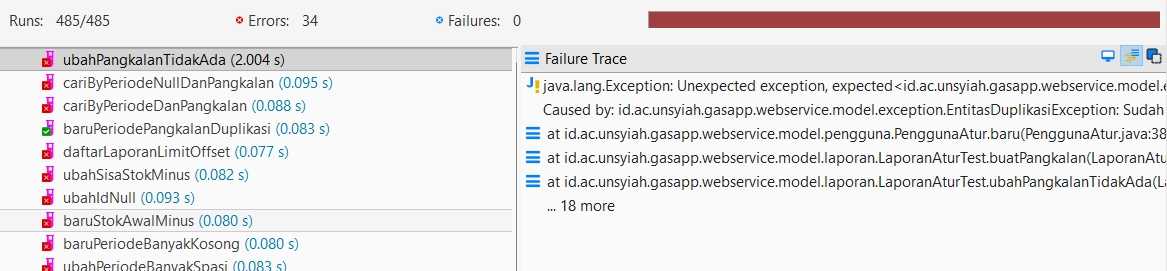
\includegraphics [width = 14cm]{gambar/kode/junit-fail}
				\caption{Pengujian JUnit Gagal}
				\label{junitFail}
			\end{figure}
	
	
	\subsection{Metode \textit{Blackbox}}
	
	Pada pengujian menggunakan metode \textit{blackbox}, aspek yang diuji adalah aspek fungsionalitas dari aplikasi tanpa melihat proses logika yang terjadi dibelakang. Berikut hasil dari pengujian ini dapat dilihat pada tabel \ref{ujiWeb} untuk aplikasi berbasis \textit{web} dan tabel \ref{ujiMobile} untuk aplikasi android.
	
	\begin{longtable}{ |c|p{3cm}|p{3cm}|p{3cm}|p{2cm}|}
	\caption{Pengujian \textit{blackbox} pada aplikasi berbasis web}
	\label{ujiWeb} \\ \hline
	\textbf{No.}                  &  \textbf{Nama Pengujian}         & \textbf{Skenario}                                       & \textbf{Luaran}              & \textbf{Hasil Pengujian} \\ \hline
	
	
	\multirow{2}{*}{1.}  & 	\multirow{2}{*}{Login Akun} & Klik \textit{link} "Login menggunakan Email Google"           & Tampil form login google yang harus diisi oleh pengguna.             & Berhasil \\ \cline{3-5}
	& & Masukkan email google dan passwordnya           & muncul halaman beranda         & Berhasil \\ \hline
	
	\multirow{3}{*}{2.}  & 	\multirow{3}{*}{Tambah Pangkalan} & Klik menu pangkalan           & Tampil daftar pangkalan yang ada.             & Berhasil \\ \cline{3-5}
	& & Klik tombol "tambah pangkalan"           & Tampil form untuk menginput data pangkalan baru.             & Berhasil \\ \cline{3-5}
	& & Masukkan data pangkalan ke dalam form dan klik tombol "simpan"           & Muncul peringatan bahwa pangkalan telah berhasil ditambah.             & Berhasil \\ \hline
	
	\multirow{4}{*}{3.}  & 	\multirow{4}{*}{Edit Pangkalan} & Klik menu pangkalan           & Tampil daftar pangkalan yang ada.             & Berhasil \\ \cline{3-5}
	& & Klik tombol "profil"           & Tampil form data pangkalan yang ter-\textit{disable} semua.             & Berhasil \\ \cline{3-5}
	& & Klik tombol "edit"           & form tadi dapat diedit             & Berhasil \\ \hline
	& & Edit data pangkalan pada form dan klik tombol "simpan"           & Muncul peringatan bahwa pangkalan telah berhasil diedit.             & Berhasil \\ \hline
	
	
	\multirow{4}{*}{4.}  & 	\multirow{4}{*}{\parbox{3cm}{\centering Tambah Rencana Pasokan Tabung}} & Klik menu pangkalan           & Tampil daftar pangkalan yang ada.             & Berhasil \\ \cline{3-5}
	& & Klik tombol "Rencana Pasokan"           & Tampil halaman daftar pasokan tabung untuk pangkalan tersebut.             & Berhasil \\ \cline{3-5}
	& & Klik tombol "tambah penerimaan"           & Muncul form untuk menginput data rencana pasokan.             & Berhasil \\ \cline{3-5}
	& & Masukkan data pasokan tabung ke dalam form dan klik tombol "simpan"     & Muncul peringatan bahwa data pasokan telah berhasil ditambah.             & Berhasil \\ \hline
	
	\multirow{2}{*}{5.}  & 	\multirow{2}{*}{Ekspor Laporan} & Klik menu data laporan          & Tampil Form Ekspor Laporan.             & Berhasil \\ \cline{3-5}
	& & Masukkan periode laporan dan milik pangkalan mana setelah itu klik tombol "Ekspor Data"     & Muncul laporan penyaluran tabung dalam bentuk file PDF.             & Berhasil \\ \hline
		
	\end{longtable}

	\pagebreak
	
	\begin{longtable}{ |c|p{3cm}|p{3cm}|p{3cm}|p{2cm}|}
		\caption{Pengujian \textit{blackbox} pada aplikasi berbasis android}
		\label{ujiMobile} \\ \hline
		\textbf{No.}                  &  \textbf{Nama Pengujian}         & \textbf{Skenario}                                       & \textbf{Luaran}              & \textbf{Hasil Pengujian} \\ \hline
		
		
		\multirow{2}{*}{1.}  & 	\multirow{2}{*}{Login Akun} & Masukkan no HP akun pangkalan yang telah terdaftar           & masuk SMS kode OTP dan  Tampil halaman verifikasi OTP         & Berhasil \\ \cline{3-5}
		& & Masukkan Kode OTP dan tekan tombol "verifikasi"           & muncul halaman beranda         & Berhasil \\ \hline
		\multirow{5}{*}{2.}  & 	\multirow{5}{*}{\parbox{3cm}{\centering Register Pelanggan}} & Klik menu "register pelanggan"           & Tampil form untuk menginput data pelanggan            & Berhasil \\ \cline{3-5}
		& & Masukkan data pelanggan ke dalam form dan klik tombol "simpan"           & Tampil halaman untuk mengupload berkas pelanggan.             & Berhasil \\ \cline{3-5}
		& &  Tekan tombol "foto diri" untuk mengambil foto diri pelanggan        & Tombol "foto diri" akan terdapat logo centang             & Berhasil \\ \cline{3-5}
		& &  Tekan tombol "foto KTP" untuk mengambil foto ktp pelanggan        & Tombol "foto KTP" akan terdapat logo centang             & Berhasil \\ \cline{3-5}
		& &  Tekan tombol "simpan" untuk menginput data pelanggan baru   & Muncul peringatan bahwa data pelanggan baru telah berhasil ditambah.             & Berhasil \\ \hline
		
		\multirow{1}{*}{3.}  & 	\multirow{1}{*}{Penjualan Tabung} & Klik menu "Penjualan Tabung"          & Tampil halaman untuk mencari pelanggan.             & Berhasil \\ \hline
		\multirow{5}{*}{} & \multirow{5}{*}{} & Masukkan nik dari pelanggan yang membeli tabung dan tekan nama pelanggan           & Tampil data detail pelanggan.             & Berhasil \\ \cline{3-5}
		& & Klik tombol "beli tabung"           & tampil halaman pilihan jumlah tabung & Berhasil
		 \\ \cline{3-5}
		& & tekan salah pilihan tabung           & Tampil halaman untuk mengupload bukti pembelian.             & Berhasil \\ \cline{3-5}
		& &  Tekan tombol "foto Bukti Pembelian" untuk mengambil foto Bukti Pembelian pelanggan        & Tombol "foto Bukti Pembelian" akan terdapat logo centang             & Berhasil \\ \cline{3-5}
		& &  Tekan tombol "simpan" untuk menginput data penjualan  & Muncul peringatan bahwa penjualan baru telah berhasil.             & Berhasil \\ \hline
		
		\multirow{4}{*}{4.}  & 	\multirow{4}{*}{\parbox{3cm}{\centering Riwayat Pembelian Tabung}} & Klik menu "Penjualan Tabung"          & Tampil halaman untuk mencari pelanggan.             & Berhasil \\ \cline{3-5}
		 & & Masukkan nik dari pelanggan yang membeli tabung dan tekan nama pelanggan           & Tampil data detail pelanggan.             & Berhasil \\ \cline{3-5}
		& & Tekan tombol "riwayat pembelian"           & tampil halaman daftar riwayat pembelian tabung & Berhasil
		\\ \hline
		& & tekan salah satu dari daftar pembelian           & Tampil halaman yang menampilkan foto bukti pembelian.             & Berhasil \\ \hline
	
		
		
		\multirow{3}{*}{5.}  & 	\multirow{3}{*}{\parbox{3cm}{\centering Verifikasi Penerimaan Pasokan Tabung}} & Klik menu "Penerimaan Tabung"           & Tampil daftar penerimaan pasokan yang ada.             & Berhasil \\ \cline{3-5}
		& & geser salah salah satu daftar penerimaan dan tekan tombol centang           & Tampil peringatan konfirmasi penerimaan tabung.             & Berhasil \\ \cline{3-5}
		& & Tekan tombol "ya"           & Muncul peringatan bahwa penerimaan tabung telah berhasil dan jumlah tabung bertambah.             & Berhasil \\ \hline
		
	\end{longtable}

	Berdasarkan tabel \ref{ujiWeb} dan tabel \ref{ujiMobile} seluruh pengujian yang telah dilakukan berhasil sehingga aplikasi web dan android sudah dapat berjalan dengan baik. 
	
	\subsection{Metode \textit{Usability Testing}}
	
	Setelah melakukan pengujian sistem, selanjutnya aplikasi akan diuji dengan pengujian \textit{Usability Testing} pada tujuh responden dan mengisi kuesioner SUS. SUS memiliki kuesioner yang terdiri dari 10 pertanyaan. Contoh dari SUS dapat dilihat pada tabel \ref{kuesioner}. \textit{Test Plan} pengujian ini dapat dilihat pada tabel \ref{test plan}.
	
		\begin{center}
		\begin{table}[H]
			\center
			\caption{\textit{Test Plan }pengujian \textit{usability} aplikasi}
			\label{test plan}
			\begin{tabular}{ |p{12cm}|  }
				\hline
				\multicolumn{1}{|c|}{\textbf{\textit{Test Plan} \textit{Usablity Testing}}} \\
				\hline
				Lokasi :
				\begin{enumerate}
					\item PT Pasha Jaya, Meuraxa
					\item Starjazz Kupi, Batoh
					\item Dhapu Kupi, Batoh
					\item Pangkalan Gas Ateuk Meunjeng
					\item Pangkalan Gas Lingke
					\item Pangkalan Gas Lampeunereut
				\end{enumerate}
				Skenario :
				\begin{enumerate}[a.]
					\item Mobile:
						\begin{enumerate}[1.]
							\item Pengguna \textit{login} kedalam aplikasi
							\item Pengguna mendaftarkan pelanggan baru
							\item Pengguna mencatat pembelian tabung 
							\item Pengguna konfirmasi penerimaan pasokan tabung
							\item Pengguna keluar dari aplikasi
							
						\end{enumerate}
					\item Web:
						\begin{enumerate}[1.]
							\item Pengguna \textit{login} kedalam aplikasi
							\item Pengguna menambahkan pangkalan baru.
							\item Pengguna menginput rencana pasokan tabung untuk pangkalan.
							\item Pengguna mencetak laporan penyaluran tabung.
							\item Pengguna keluar dari aplikasi
							
						\end{enumerate}
				\end{enumerate}
				 \\
				\hline
			\end{tabular}
		\end{table}
	\end{center}

	\begin{center}
	\begin{tabular}{ |p{12cm}|  }
		\hline
		Alat   : \textit{Smartphone} Android untuk menggunakan aplikasi dan laptop untuk menggunakan aplikasi berbasis web\\
		Hasil : Hasil Pengujian SUS terdapat pada Tabel \ref{hasilSusAgen} dan Tabel \ref{hasilSusPangkalan}\\
		\hline
	\end{tabular}
\end{center}

\begin{table}[H]
	\center
	\caption{Hasil Pengujian SUS pada Aplikasi Berbasis Web untuk Agen.}
	\label{hasilSusAgen}
	\begin{tabular}{|c|l|l|l|l|l|l|l|l|l|l|l|}
		\hline
		\multirow{2}{*}{Nama} & \multicolumn{10}{c|}{Skor Untuk Tiap Pertanyaan} &  \multirow{2}{0.5cm}{Jml} \\ \cline{2-11} 
		&1 &2  &3 &4 &5 &6 &7 &8 &9 &10& \\
		\hline
		User 1 &8 &8 &8 &6 &8 &10 &10 &6 &10 &6 &80 \\ 
		\hline
		User 2 &8 &6 &8 &8 &8 &8 &10 &8 &6 &6 &76 \\ 
		\hline
		User 3 &8 &10 &10 &4 &8 &10 &10 &10 &10 &8 &88 \\ 
		\hline
		User 4 &8 &6 &10 &8 &8 &8 &10 &8 &8 &8 &82 \\ 
		\hline
		User 5 &8 &6 &8 &8 &6 &8 &8 &6 &8 &8 &74 \\ 
		\hline
		User 6 &6 &8 &6 &8 &8 &8 &8 &6 &8 &8 &74 \\ 
		\hline
		User 7 &6 &6 &8 &8 &10 &6 &6 &10 &8 &8 &76 \\ 
		\hline
		User 8 &8 &8 &10 &6 &10 &10 &8 &6 &6 &6 &80 \\ 
		\hline
	\end{tabular}
\end{table}

\begin{table}[H]
	\center
	\caption{Hasil Pengujian SUS pada Aplikasi Berbasis Android untuk Pangkalan.}
	\label{hasilSusPangkalan}
	\begin{tabular}{|c|l|l|l|l|l|l|l|l|l|l|l|}
		\hline
		\multirow{2}{*}{Nama} & \multicolumn{10}{c|}{Skor Untuk Tiap Pertanyaan} &  \multirow{2}{0.5cm}{Jml} \\ \cline{2-11} 
		&1 &2  &3 &4 &5 &6 &7 &8 &9 &10& \\
		\hline
		User 1 &10 &6 &10 &8 &10 &10 &10 &8 &10 &6 &88 \\ 
		\hline
		User 2 &8 &6 &8 &8 &4 &8 &8 &8 &8 &6 &72 \\ 
		\hline
		User 3 &8 &10 &8 &6 &10 &10 &10 &10 &8 &6 &86 \\ 
		\hline
		User 4 &10 &8 &8 &6 &8 &8 &8 &10 &8 &6 &80 \\ 
		\hline
		User 5 &8 &6 &6 &8 &8 &8 &8 &8 &6 &8 &74 \\ 
		\hline
		User 6 &6 &6 &8 &10 &8 &8 &10 &8 &8 &6 &78 \\ 
		\hline
		User 7 &8 &10 &6 &6 &10 &6 &6 &8 &8 &6 &74 \\ 
		\hline
		User 8 &8 &8 &8 &6 &6 &6 &6 &8 &8 &6 &70 \\ 
		\hline
	\end{tabular}
\end{table}

Dari hasil pengujian usability diperoleh skor yang dihitung dari nilai rata-rata seluruh responden untuk aplikasi berbasis web untuk Agen yaitu sebesar 78 dan aplikasi berbasis android untuk Pangkalan sebesar 77. Maka untuk mendapatkan interpretasi skor tersebut, dihitung persentase pencapaian dengan rumus berikut. 

\[persentase = \frac{nilai Total}{nilai Maximum}\times100\]
\[persentase Aplikasi Web = \frac{78}{100}\times100=78\%\]
\[persentase Aplikasi Android = \frac{77}{100}\times100=77\%\]

Persentase pencapaian untuk aplikasi ini yaitu 78\% untuk aplikasi web dan 77\% untuk aplikasi android. Kemudian dilakukan komparasi nilai persentase pencapaian dengan interpretasi skor. Aplikasi-aplikasi ini berada pada rentang 61-80\% dengan interpretasi skor “Layak”. Berdasarkan hasil tersebut, dapat disimpulkan bahwa aplikasi-aplikasi ini memiliki fitur yang baik dan sesuai dengan kebutuhan setiap kelompok pengguna serta dapat digunakan untuk membantu dalam hal laporan penyaluran gas LPG 3 Kg.  

Selama pengujian usability berlangsung dilakukan pula penghitungan terhadap waktu pengerjaan (\textit{time on task}) dan kesalahan pengguna dalam menyelesaikan tugas-tugas \textit{(task error)} yang diberikan. Penghitungan\textit{ \textit{time on task}} dilakukan untuk mengetahui berapa lama waktu yang dibutuhkan pengguna untuk mengerjakan tugas yang diberikan dan diukur dalam satuan detik (s). Hasil dari penghitungan \textit{time on task} untuk aplikasi untuk agen dapat dilihat pada tabel \ref{timeOnTaskAgen} dan untuk pangkalan dapat dilihat pada tabel \ref{timeOnTaskPangkalan}. 

\begin{table}[H]
	\center
	\caption{\textit{Time On Task} Pengujian Aplikasi Berbasis Web untuk Agen.}
	\label{timeOnTaskAgen}
	\begin{tabular}{|c|l|l|l|l|l|}
		\hline
		\multirow{2}{*}{Nama} & \multicolumn{5}{c|}{Tugas (s)} \\ \cline{2-6} 
		&1 &2  &3 &4 &5  \\
		\hline
		User 1 &10 &20 &27 &15 &6  \\ 
		\hline
		User 2 &12 &22 &29 &16 &5  \\ 
		\hline
		User 3 &8 &19 &28 &15 &5  \\ 
		\hline
		User 4 &9 &20 &23 &18 &7  \\ 
		\hline
		User 5 &8 &19 &24 &17 &8  \\ 
		\hline
		User 6 &10 &23 &25 &16 &8 \\ 
		\hline
		User 7 &12 &20 &23 &15 &8  \\ 
		\hline
		User 8 &10 &21 &26 &15 &8  \\ 
		\hline
		Total(s)  &79 &164 &205 &127 &53 \\ 
		\hline
		Rata-Rata(s)  &10 &21 &26 &16 &7  \\ 
		\hline
	\end{tabular}
\end{table}

\begin{table}[H]
	\center
	\caption{\textit{Time On Task} Pengujian Aplikasi Berbasis Android untuk Pangkalan.}
	\label{timeOnTaskPangkalan}
	\begin{tabular}{|c|l|l|l|l|l|}
		\hline
		\multirow{2}{*}{Nama} & \multicolumn{5}{c|}{Tugas (s)} \\ \cline{2-6} 
		&1 &2  &3 &4 &5  \\
		\hline
		User 1 &12 &20 &24 &15 &7  \\ 
		\hline
		User 2 &11 &22 &26 &15 &8  \\ 
		\hline
		User 3 &10 &21 &27 &14 &8  \\ 
		\hline
		User 4 &9 &19 &24 &16 &10  \\ 
		\hline
		User 5 &12 &23 &25 &14 &9  \\ 
		\hline
		User 6 &10 &19 &28 &17 &10 \\ 
		\hline
		User 7 &9 &23 &27 &16 &7  \\ 
		\hline
		User 8 &10 &22 &21 &19 &9  \\ 
		\hline
		Total(s)  &83 &169 &202 &126 &68 \\ 
		\hline
		Rata-Rata(s)  &11 &22 &26 &16 &9  \\ 
		\hline
	\end{tabular}
\end{table}

Tugas 2 dan 3 pada tabel \ref{timeOnTaskAgen} dibutuhkan waktu yang sedikit lebih lama ketimbang tugas lainnya karena ada beberapa \textit{form} yang harus diisikan oleh \textit{user}. Begitu juga tugas 2 dan 3 pada tabel \ref{timeOnTaskPangkalan} dibutuhkan waktu agak lama untuk mengisi \textit{form} dan juga mengunggah data foto.

Penghitungan \textit{task error} dilakukan untuk mengetahui seberapa banyak kesalahan yang dilakukan pengguna dalam mengerjakan tugas yang diberikan.Hasil dari penghitungan nya  dapat dilihat pada tabel \ref{taskErrorAgen} untuk agen dan table \ref{taskErrorPangkalan} untuk pangkalan. 
\begin{table}[H]
	\center
	\caption{\textit{Task Error} Pengujian Aplikasi Berbasis web untuk Agen.}
	\label{taskErrorAgen}
	\begin{tabular}{|c|l|l|l|l|l|l|}
		\hline
		\multirow{2}{*}{Nama} & \multicolumn{5}{c|}{Tugas} &  \multirow{2}{0.5cm}{Jml} \\ \cline{2-6} 
		&1 &2  &3 &4 &5& \\
		\hline
		User 1 &0 &0 &0 &0 &0 &0 \\ 
		\hline
		User 2 &0 &0 &1 &0 &0 &1  \\ 
		\hline
		User 3 &0 &0 &0 &0 &0 &0  \\ 
		\hline
		User 4 &0 &0 &0 &0 &0 &0  \\ 
		\hline
		User 5 &0 &0 &0 &1 &0 &1  \\ 
		\hline
		User 6 &0 &0 &1 &1 &1 &2  \\ 
		\hline
		User 7 &0 &0 &0 &0 &0 &0 \\ 
		\hline
		User 8 &0 &0 &1 &0 &0 &1 \\ 
		\hline
		Total(s)  &0 &0 &3 &2 &0 &5 \\ 
		\hline
	\end{tabular}
\end{table}

\begin{table}[H]
	\center
	\caption{\textit{Task Error} Pengujian Aplikasi Berbasis android untuk Pangkalan.}
	\label{taskErrorPangkalan}
	\begin{tabular}{|c|l|l|l|l|l|l|}
		\hline
		\multirow{2}{*}{Nama} & \multicolumn{5}{c|}{Tugas} &  \multirow{2}{0.5cm}{Jml} \\ \cline{2-6} 
		&1 &2  &3 &4 &5& \\
		\hline
		User 1 &0 &0 &1 &0 &0 &1 \\ 
		\hline
		User 2 &0 &0 &1 &0 &0 &1  \\ 
		\hline
		User 3 &0 &0 &0 &0 &0 &0  \\ 
		\hline
		User 4 &0 &0 &0 &0 &0 &0  \\ 
		\hline
		User 5 &0 &1 &0 &0 &0 &1  \\ 
		\hline
		User 6 &0 &1 &1 &0 &0 &2  \\ 
		\hline
		User 7 &0 &0 &0 &0 &0 &0 \\ 
		\hline
		User 8 &0 &0 &0 &0 &1 &1 \\ 
		\hline
		Total(s)  &0 &2 &3 &0 &1 &6 \\ 
		\hline
	\end{tabular}
\end{table}
Tabel \ref{taskErrorAgen} dapat dilihat bahwa tugas 3 dan 4 sering terjadi \textit{task error}. Berdasarkan \textit{think aloud} yang dilakukan saat proses usability hal ini terjadi karena \textit{user} agen belum terbiasa dengan alur aplikasi. Sedangkan pada tabel \ref{taskErrorPangkalan} dapat dilihat bahwa tugas tugas 2 dan 3 sering terjadi \textit{task error}, ini  terjadi karena \textit{user} pangkalan belum terbiasa dengan tampilan aplikasi pada saat mengambil gambar.
Aplikasi ini dirancang dan dibangun dan diuji untuk pertama kalinya, sehingga pasti memiliki kritik  yang diberikan saat proses \textit{usability testing} dilakukan. Berikut beberapa kritik yang diberikan oleh pengguna : \newline \newline
Kritik :
\begin{enumerate}
	\item Fitur untuk impor data penerimaan pasokan sekaligus via CSV untuk pengembangan selanjutnya.
	\item Fitur untuk melakukan pemblokiran pada pelanggan yang telah melewati batas pembelian untuk pengembangan selanjutnya.
	\item Tampilan pada saat mengambil gambar di \textit{improve} lagi, tapi untuk fitur-fitur dasarnya sudah cukup lumayan.
	\item UX harus di \textit{improve} lagi untuk mempercepat proses validasi pada proses pembelian tabung dikarenakan adanya antrian pada saat membeli tabung.
	
\end{enumerate}  
	
% Baris ini digunakan untuk membantu dalam melakukan sitasi.
% Karena diapit dengan comment, maka baris ini akan diabaikan
% oleh compiler LaTeX.
\begin{comment}
\bibliography{daftar-pustaka}
\end{comment}